%% For double-blind review submission, w/o CCS and ACM Reference (max submission space)
\documentclass[acmsmall,review,anonymous,screen]{acmart}\settopmatter{printfolios=true,printccs=true,printacmref=true}
%% For double-blind review submission, w/ CCS and ACM Reference
%\documentclass[acmsmall,review,anonymous]{acmart}\settopmatter{printfolios=true}
%% For single-blind review submission, w/o CCS and ACM Reference (max submission space)
%\documentclass[acmsmall,review]{acmart}\settopmatter{printfolios=true,printccs=false,printacmref=false}
%% For single-blind review submission, w/ CCS and ACM Reference
%\documentclass[acmsmall,review]{acmart}\settopmatter{printfolios=true}
%% For final camera-ready submission, w/ required CCS and ACM Reference
%\documentclass[acmsmall]{acmart}\settopmatter{}


%% Journal information
%% Supplied to authors by publisher for camera-ready submission;
%% use defaults for review submission.
\acmJournal{PACMPL}
\acmVolume{1}
\acmNumber{POPL} % CONF = POPL or ICFP or OOPSLA
\acmArticle{1}
\acmYear{2023}
\acmMonth{1}
\acmDOI{} % \acmDOI{10.1145/nnnnnnn.nnnnnnn}
\startPage{1}

%% Copyright information
%% Supplied to authors (based on authors' rights management selection;
%% see authors.acm.org) by publisher for camera-ready submission;
%% use 'none' for review submission.
\setcopyright{none}
%\setcopyright{acmcopyright}
%\setcopyright{acmlicensed}
%\setcopyright{rightsretained}
%\copyrightyear{2018}           %% If different from \acmYear

%% Bibliography style
\bibliographystyle{ACM-Reference-Format}
%% Citation style
%% Note: author/year citations are required for papers published as an
%% issue of PACMPL.
\citestyle{acmauthoryear}   %% For author/year citations


%%%%%%%%%%%%%%%%%%%%%%%%%%%%%%%%%%%%%%%%%%%%%%%%%%%%%%%%%%%%%%%%%%%%%%
%% Note: Authors migrating a paper from PACMPL format to traditional
%% SIGPLAN proceedings format must update the '\documentclass' and
%% topmatter commands above; see 'acmart-sigplanproc-template.tex'.
%%%%%%%%%%%%%%%%%%%%%%%%%%%%%%%%%%%%%%%%%%%%%%%%%%%%%%%%%%%%%%%%%%%%%%


%% Some recommended packages.
\usepackage{booktabs}   %% For formal tables:
                        %% http://ctan.org/pkg/booktabs
\usepackage{subcaption} %% For complex figures with subfigures/subcaptions
                        %% http://ctan.org/pkg/subcaption



\usepackage{amsmath,empheq,fancybox}
\usepackage{paralist}
\usepackage{url}
\usepackage{color}
\usepackage{textcomp,listings}
\usepackage{array}
\usepackage{mymacros}
\usepackage{microtype}
\usepackage{listings}
\usepackage{csquotes}
\usepackage{proof}
\usepackage[capitalise]{cleveref}
\usepackage{algorithm2e}      
\usepackage{multirow}
\usepackage{mathpartir}
\usepackage{amsthm}
\usepackage{numprint}
\usepackage{ebproof}
\usepackage[makeroom]{cancel}

\usepackage{mathtools} % Bonus

\usepackage{enumitem}


\theoremstyle{definition}
\newtheorem{definition}{Definition}[section]
\newtheorem{example}{Example}[section]

\newlist{constraints}{enumerate}{3}
\setlist[constraints,1]{%
    label=\sffamily{(\roman*):},
    ref=\normalfont{Constraint (\roman*)},
    wide,itemsep=0pt,topsep=0pt
}    
\crefname{constraintsi}{}{}
\Crefname{constraintsi}{}{}


\lstset{
    columns=fullflexible,
    showspaces=false,
    showtabs=false,
    breaklines=true,
    showstringspaces=false,
    breakatwhitespace=true,
    escapeinside={(*@}{@*)},
    commentstyle=\color{greencomments},
    keywordstyle=\color{bluekeywords},
    stringstyle=\color{redstrings},
    numberstyle=\color{graynumbers},
    basicstyle=\ttfamily\small,
    framesep=12pt,
    xleftmargin=12pt,
    tabsize=4,
    captionpos=b
}


\newif\ifcomments
\commentstrue
\newif\ifoutline
\outlinetrue

\newcommand{\contents}[1]{\ifoutline{\color{blue}
    \begin{itemize}
    #1
    \end{itemize}
  }\fi}

\allowdisplaybreaks[1]


\begin{document}

%% Title information
\title{A Constraint Solving Approach to Parikh Images of Regular Languages}
                                        %% when present, will be used in
                                        %% header instead of Full Title.
%% Author information
%% Contents and number of authors suppressed with 'anonymous'.
%% Each author should be introduced by \author, followed by
%% \authornote (optional), \orcid (optional), \affiliation, and
%% \email.
%% An author may have multiple affiliations and/or emails; repeat the
%% appropriate command.
%% Many elements are not rendered, but should be provided for metadata
%% extraction tools.

%% Author with single affiliation.
\author{First1 Last1}
\authornote{with author1 note}          %% \authornote is optional;
                                        %% can be repeated if necessary
\orcid{nnnn-nnnn-nnnn-nnnn}             %% \orcid is optional
\affiliation{
  \position{Position1}
  \department{Department1}              %% \department is recommended
  \institution{Institution1}            %% \institution is required
  \streetaddress{Street1 Address1}
  \city{City1}
  \state{State1}
  \postcode{Post-Code1}
  \country{Country1}                    %% \country is recommended
}
\email{first1.last1@inst1.edu}          %% \email is recommended

%% Author with two affiliations and emails.
\author{First2 Last2}
\authornote{with author2 note}          %% \authornote is optional;
                                        %% can be repeated if necessary
\orcid{nnnn-nnnn-nnnn-nnnn}             %% \orcid is optional
\affiliation{
  \position{Position2a}
  \department{Department2a}             %% \department is recommended
  \institution{Institution2a}           %% \institution is required
  \streetaddress{Street2a Address2a}
  \city{City2a}
  \state{State2a}
  \postcode{Post-Code2a}
  \country{Country2a}                   %% \country is recommended
}
\email{first2.last2@inst2a.com}         %% \email is recommended
\affiliation{
  \position{Position2b}
  \department{Department2b}             %% \department is recommended
  \institution{Institution2b}           %% \institution is required
  \streetaddress{Street3b Address2b}
  \city{City2b}
  \state{State2b}
  \postcode{Post-Code2b}
  \country{Country2b}                   %% \country is recommended
}
\email{first2.last2@inst2b.org}         %% \email is recommended


%% Abstract
%% Note: \begin{abstract}...\end{abstract} environment must come
%% before \maketitle command
\begin{abstract}
  A common problem in string constraint solvers is computing the Parikh image, a
   set of linear equations that describe all possible combinations of character
   counts in strings of a given language. Automata-based string solvers
   frequently need to compute the Parikh image of large products (intersections)
   of nondeterministic automata, which in many operations is both prohibitively
   slow and memory-intensive. We contribute a novel understanding of how Parikh
   maps can be tackled as a constraint solving problem to solve real-world
   constraints stemming from functions on regular languages, most notably the
   length constraint. Furthermore, we show how this formulation can be
   efficiently implemented as a calculus, \Calculus{}, in an automated theorem
   prover supporting Presburger logic.  We implement \Calculus{} in a tool
   called \Catra{}, and evaluate it on constraints produced by the
   \OstrichPlus{} string constraint solver when solving Parikh automata
   intersection problems produced when solving standard string constraint
   benchmarks involving string length constraints. We show that our solution
   strictly outperforms the standard approach described
   in~\citeauthor{generate-parikh-image} as well as the over-approximating
   method recently described by~\citeauthor{approximate-parikh} by a wide
   marigin, and for realistic timeouts for constraint solving also the~\Nuxmv{}
   model checker.
\end{abstract}


%% 2012 ACM Computing Classification System (CSS) concepts
%% Generate at 'http://dl.acm.org/ccs/ccs.cfm'.
\begin{CCSXML}
  <ccs2012>
  <concept>
  <concept_id>10003752.10003766.10003773.10003775</concept_id>
  <concept_desc>Theory of computation~Quantitative automata</concept_desc>
  <concept_significance>500</concept_significance>
  </concept>
  <concept>
  <concept_id>10003752.10003766.10003776</concept_id>
  <concept_desc>Theory of computation~Regular languages</concept_desc>
  <concept_significance>300</concept_significance>
  </concept>
  <concept>
  <concept_id>10003752.10003790.10003794</concept_id>
  <concept_desc>Theory of computation~Automated reasoning</concept_desc>
  <concept_significance>500</concept_significance>
  </concept>
  <concept>
  <concept_id>10003752.10010124.10010138.10010142</concept_id>
  <concept_desc>Theory of computation~Program verification</concept_desc>
  <concept_significance>300</concept_significance>
  </concept>
  <concept>
  <concept_id>10003752.10003790.10011192</concept_id>
  <concept_desc>Theory of computation~Verification by model checking</concept_desc>
  <concept_significance>300</concept_significance>
  </concept>
  </ccs2012>  
\end{CCSXML}

\ccsdesc[500]{Theory of computation~Quantitative automata}
\ccsdesc[300]{Theory of computation~Regular languages}
\ccsdesc[500]{Theory of computation~Automated reasoning}
\ccsdesc[300]{Theory of computation~Program verification}
\ccsdesc[300]{Theory of computation~Verification by model checking}
%% End of generated code


%% Keywords
%% comma separated list
\keywords{Parikh images, string solvers, model checking}  %% \keywords are mandatory in final camera-ready submission


%% \maketitle
%% Note: \maketitle command must come after title commands, author
%% commands, abstract environment, Computing Classification System
%% environment and commands, and keywords command.
\maketitle


\section{Introduction}\label{sec:introduction}
The Parikh image is a characterisation of formal languages in terms of their
character counts. Given a language over an alphabet~$\{a_1, \ldots, a_k\}$, the
Parikh image is a set of $k$-dimensional vectors that contains some
vector~$\VectorLiteral{m_1, m_2, \ldots, m_k}$ if and only if the formal
language contains a word in which each $a_i$ occurs $m_i$ times. It is a
classical result that the Parikh image of every context-free language (and,
thus, also of every regular language) is a semilinear set~\cite{parikh-theorem},
i.e., Presburger-definable.

Parikh images play a central role in many automata-based algorithms, for
instance and notably in today's string solvers, which often have to process
constraints that combine regular language membership with word length. To decide
whether a simple formula like $x \in \Language_1 \wedge y \in \Language_2 \wedge
|x| > |y|$, with string variables~$x, y$ and regular languages~$\Language_1,
\Language_2$, is satisfiable, it is necessary to reason about the sets of word
lengths induced by $\Language_1, \Language_2$, which are special cases of the
Parikh image.  This required combined reasoning about strings and string length
has long been identified as a major bottleneck in string solvers
\cite{DBLP:conf/cav/AbdullaACHRRS15,length-aware-solver,approximate-parikh,DBLP:journals/corr/BerzishZG17}.
Other string solvers make use of Parikh automata~\cite{parikh-automata}, and
thus Parikh images in the general case, to handle operations including
\verb!str.substr!  and \verb!str.at!, which comes at an even higher price in
terms of computational complexity~\cite{ostrich-plus}.


It is possible to compute an existential Presburger formula describing the
Parikh image of any context-free language in linear
time~\cite{generate-parikh-image}; for the special case of regular languages,
this result was also stated in \cite{muscholl-linear}. While theoretically
elegant, this construction has several disadvantages, often making it
unpractical for integration into algorithms. Firstly, the constructed Presburger
formula contains a linear number of existential quantifiers in the size of the
considered grammar, as well as complex Boolean structure, which is needed to
express the connectedness of sets of productions considered in the construction.
Eliminating those quantifiers to obtain a quantifier-free representation of the
Parikh image has exponential complexity~\cite{DBLP:conf/issac/Weispfenning97},
and is often impossible in reasonable time. Just solving the Parikh image
membership problem is NP-complete, as it corresponds to computing a satisfying
assignment of the existential Presburger formula, and taxing for solvers as
well~\cite{ostrich-plus}.

Secondly, in applications involving regular languages, it is typically necessary
to consider the Parikh image not only of a single automaton, but of the
intersection of multiple automata. This problem arises in string solvers in
particular, as conjunctions of string constraints lead to the computation of
length images of products (intersections) of regular languages represented as
finite automata. Applying the approach in~\cite{generate-parikh-image} would in
this case require the eager computation of the product before its length image,
and result in an existential Presburger formula of exponential size (in the
number of automata). In several instances we have observed while solving
real-world string constraints, the computation of the product of automata
exhausts the memory of any machine available due to the exponential blow-up in
size of the product, quickly becoming intractable as the number of automata in
the product increases. The current best published mitigation for this problem is
an over-approximation that works by approximating the Parikh image of a product
of automata to be the conjunction of the image of the individual automata of the
product \cite{approximate-parikh}. This approach only works for unsatisfiable
instances, and comes with a harsh penalty for satisfiable instances.

Addressing these concerns, we have developed a calculus for Parikh images of
products of regular languages that we call \Calculus{}. It allows us to
interleave the computation of arbitrarily deep products of automata with the
product's Parikh image, and is generalised to an arbitrary homomorphism over
automata labels, including string lengths. This enables us to let both
calculations inform each other, eliminating unnecessary work, and pruning the
size of the partial products considered in the computation for a smaller memory
footprint. Moreover, the method can be used iteratively to tackle smaller chunks
of the product incrementally, thereby decreasing the memory footprint.

The key ideas of \Calculus{} is a combination of problem-aware case splitting,
lazy enforcement of automata connectivity, and lazy computation of products. In
essence, we use constraint-based methods to efficiently enforce the constraints
associated with computing Parikh images of regular languages.

We implement \Calculus{} as a plug-in theory for the \Princess{} automated
theorem prover. \Fudge{Others} have integrated it into the similarly
\Princess{}-backed string constraint solver \OstrichPlus{}, where it is used to
handle constraints that use cost-enriched automata, as described in
\cite{ostrich-plus}.

We additionally wrap the Parikh image solver as a stand-alone tool, \Catra.
\Catra{} also supports a variant of the approximate method of
\cite{approximate-parikh}, its fall-back variant adapted
from~\cite{generate-parikh-image}, and an adapter for the \Nuxmv{} model
checker~\cite{nuxmv}. Using \Catra, we compare \Calculus{} to the other two
back-ends on \NrBenchmarks{} distinct Parikh automata intersection problems
generated by \OstrichPlus{} when solving the PyEx string constraint benchmark
suite involving string length constraints \cite{pyex}.

In summary, we contribute:
\begin{itemize}
    \item The \Calculus{} calculus to efficiently compute (a homomorphism on)
          the Parikh image of products of Parikh automata.
    \item Experiments illustrating the performance of \Calculus{} on real-world
    examples from string solving, including \NrBenchmarks{} instances in a
    standardised format made available for future study.
    \item The \Catra{} tool for solving such instances, containing an
    implementation of \Calculus{}, the over-approximation described
    in~\cite{approximate-parikh}, and an adapter for the~\Nuxmv{} model
    checker~\cite{nuxmv}.
    \item Suggestions for how to efficiently implement \Calculus{} in a modern
    automated theorem prover, including strategies for case splitting, clause
    learning, and constraint propagation for connectedness.
\end{itemize}

\subsection{Related Work}

The problem of computing constraints on Parikh images over products of regular
languages under a given commutative homomorphism amounts to solving products of
Parikh automata. Parikh automata are regular automata extended with integer
counters with given increments and decrements for each transition, where we
allow checking a set of linear constraints on the final values of the counters
(but not their intermittent values) \cite{parikh-automata}. Parikh automata
without constraints on the final values on their registers are also sometimes
called cost-enriched automata, weighted automata or counter automata, depending
on exact definitions and side-constraints. The decision problem tackled in this
paper, determining the emptiness of an intersection of Parikh automata, was
recently shown to be PSPACE-complete~\cite{graph-queries}.

Parikh image computations as well as Parikh automata feature extensively in
string solvers, including as mentioned above \Ostrich{} and \OstrichPlus{}
\cite{ostrich,ostrich-plus}, but also forms the basis of Trau~\cite{trau-pldi},
and occurs in \textsc{Sloth}~\cite{sloth}. Parikh images frequently appear when
introducing cardinality constraints like length or string indexing. The
state-of-the-art approach to handling Parikh image computation is to
over-approximate the Parikh image of a product of $k$~automata
$\ParikhMap(\Language(\Automaton_1) \cap \ldots \cap \Language(\Automaton_k))$
with the conjunction of the automata's Parikh maps, $\bigwedge_{i=1}^{k}
\ParikhMap(\Automaton_i)$. This approach works only for unsatisfiable instances,
and will require falling back to computing the product of the automata before
using the standard approach for finding its image originally presented
in~\cite{generate-parikh-image}.

% @Philipp: please verify that this is not a lie!
The problem and our calculus, \Calculus{}, takes a similar approach to the work
of \citeauthor{symbolic-boolean-derivatives}, who present an orthogonal calculus
for handling a similar blow-up in complexity resulting from Boolean combinations
of regular automata in SMT string solvers \cite{symbolic-boolean-derivatives}.
In addition to presenting a decision procedure for lazily dispatching
constraints, we similarly also allow for symbolic labelling of automata to
handle large Unicode alphabets.

Outside of string solvers, Parikh automata have been proposed as the basis of
queries~\cite{graph-queries}, and for solving cardinalities in model checking
problems involving epistemic logic~\cite{epistemic-logic}.

Many other generalisations of the Parikh image than the projections we use here
have been studied. Prominent examples include generalising the Parikh map to
segments of a fixed length \cite{KARHUMAKI1980155} and the more general Parikh
matrix, which gives more information about a word than the standard Parikh image
\cite{parikh-matrix}. Another notable generalisation is the p-vector, introduced
in~\cite{infinite-words}, which denotes the position of each letter in the word
rather than the number of their occurrences and allows for generalisations into
infinite alphabets. All of these in some sense extend the Parikh map. By
contrast, the main utility of the formulation introduced here is that it allows
us to \emph{remove} something, thereby potentialy obtaining an easier problem.

\section{An Intuition for Our Approach}\label{sec:intuition}
\begin{figure}[h]
    \centering 
  \begin{subfigure}[b]{0.5\textwidth}
    \centering
    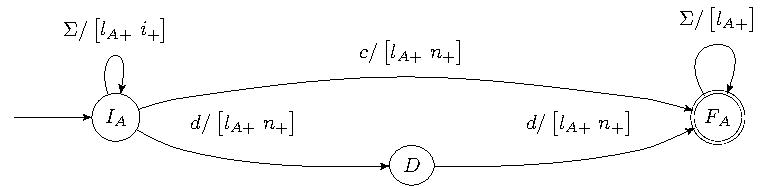
\includegraphics[scale=\autscale]{a}
    \caption{The automaton $A'$, whose Parikh registers count the length of the
    string accepted by the automaton (register $l_A$), the start offset of the
    substring ($i$) and length ($n$) of the substring matching
    $\Regex{c\RegexOr{}dd}$. Note the symbolic transitions in the starting and
    accepting states matching any symbol in the alphabet!}\label{fig:aut_a}
      %\Description[SHORT]{LONG}
  \end{subfigure}
  \begin{subfigure}[b]{0.5\textwidth}
    \centering
    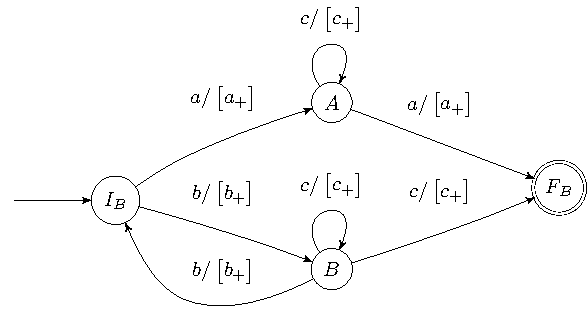
\includegraphics[scale=\autscale]{b}
    \caption{The automaton $B$, where the Parikh registers count the length of
    the string in register $l_B$.}\label{fig:aut_b}
      %\Description[SHORT]{LONG}
  \end{subfigure}
  \caption{The collection of automata we use as running
  examples}\label{fig:examples}
\end{figure}


In this section we will introduce an intuition for how a string constraint
problem in an automata-based solver like \OstrichPlus{} is translated to a
Parikh automata intersection problem and solved using \Calculus{}. First, by a
Parikh automaton we mean a standard non-deterministic finite automaton (NFA)
with a set of integer registers (Parikh registers) that are incremented (or
decremented) at each transition. In the automata of \cref{fig:examples}, we will
use the notation $a / \begin{bmatrix} x_+ \end{bmatrix}$ to mean that a
transition reads an input character $a$ and increments register $x$ by one. We
will omit zero-valued increments and assume that all registers are scoped to
their automaton. The increments are usually represented as a vector (hence the
brackets), but as it is mostly sparse here, we use the symbolic notation
$\begin{bmatrix} x_{1+} \end{bmatrix}$ rather than the more cumbersome $\left[
0, 1,  0 , \ldots, 0 \right]$.

Note that the labels of transitions can be ranges of characters with $\Sigma$
representing any character in the alphabet.

We use PCRE regular expression notation here and throughout the paper, writing
them $\Regex{\texttt{like this}}$. This means that $\RegexOr{}$ is alternation,
$\mathtt{*}$ the Kleene star, and $\mathtt{.}$, matches any single character.

For the length of a string $s$, we write $\Length{s}$.

\begin{example}\label{ex:string-constraints} Consider the following set of
    string constraints:
\begin{constraints}
    \item\label{const:s1-in-c-dd} $s_1 \in \Language(\Regex{c\RegexOr{}dd})$.
    \item\label{const:s2-in-b} $s_2 \in \Language(B)$, the language accepted by
    automaton~$B$ of \cref{fig:aut_b}.
    \item\label{const:s1-substring} $s_1 = \Substring(s_2, i, n)$, that is $s_1$ is an
    $n$-length substring of $s_2$ starting at offset $i$.
    \item\label{const:more-inside-than-before} $n > i$, that is what comes
    before $s_1$ in $s_2$ is shorter than $s_1$.
    \item\label{const:something-before-and-after} $i > 0 \land \Length{s_2} -i -n > 0$, that
    is there is at least one character in $s_2$ after $s_1$.
\end{constraints}
\end{example}

To solve \cref{ex:string-constraints} using \Calculus{} in a theorem proving
context, \cref{const:s1-in-c-dd,const:s2-in-b,const:s1-substring} can be
translated to the product of Parikh automata $B \times A'$, where $A'$
(\cref{fig:aut_a}) is the Parikh automata obtained by applying the encoding of
$\Substring$ described in \cite{ostrich-plus}. That description can then be used
to obtain values for the subsstring offsets $i, n$.

Intuitively, \cref{ex:string-constraints} are unsatisfiable. By inspecting the
automata, we realise that the path using $\Char{dd}$ in $A'$ is unusable since
are no $\Char{d}$-labelled transitions in $B$. This means that $s_1 = \Char{c}$,
and thus $n = 1$. That means that \cref{const:more-inside-than-before} implies
that $i = 0$. However, no path through $B$ passes by a $\Char{c}$ without a
preceding character. Therefore, already
\cref{const:s1-in-c-dd,const:s1-in-c-dd,const:s1-substring,const:more-inside-than-before}
together are unsatisfiable.


Our approach to the computation of the Parikh image (and therefore the solution
to the intersection problem posed by \cref{ex:string-constraints}) consists of
two applications of laziness; late computation of products of automata, and lazy
enforcement of connectivity constraints. Both are in contrast to the eager
approach to finding the Parikh image described in~\cite{generate-parikh-image},
that would have started by computing the product $A' \times B$, translated it to
a Presburger formula with $i, n$ etc as free variables, and then plugged in
\cref{const:more-inside-than-before,const:something-before-and-after}.

Starting with an interactive theorem prover and the goal of solving the Parikh
automata intersection problem, we associate each transition $\Transition$ of
$A'$ and $B$ with a fresh nonnegative integer variable from,
$\TransitionVar_\Transition$, identically to \cite{generate-parikh-image}. These
variables represent how many times each transition is taken. Hence, the final
counter value for counters $r_1, \ldots, r_k$ of each automaton is the
element-wise sum:
\begin{equation}\label{eq:counter-sums}
\begin{bmatrix} 
  r_1 \\
  \vdots\\
  r_k \\
\end{bmatrix} = \sum_\Transition \TransitionVar_\Transition \cdot 
  \IncrementVec_\Transition \text{ where $\IncrementVec_\Transition$ are the increments of transition $\Transition$}.
\end{equation}

We proceed by adding linear constraints requiring transition variables to
represent a flow through their automaton by adding linear constraints stating
that the number of incoming transitions is equal to the number of outgoing ones.
E.g. state $B$ would have the sum $\cancel{x_{\Tuple{B, \Char{c}, B}}} +
x_{\Tuple{I_B, \Char{b}, B}} = \cancel{x_{\Tuple{B, \Char{c}, B}}}  +
x_{\Tuple{B, \Char{c}, F_B}} + x_{\Tuple{B, \Char{b}, I_B}}$ where we let
$x_{\Tuple{q, l, c'}}$ refer to the integer variable associated with a
transition from state $q$ to state $q'$ with label $l$. Note that the self-loop
cancels itself out. This means that for automata where a loop can become
unreachable, additional constraints would be required to ensure reachability.
However, being lazy, we put off that work until later.

\begin{figure}[h]
  \centering 
  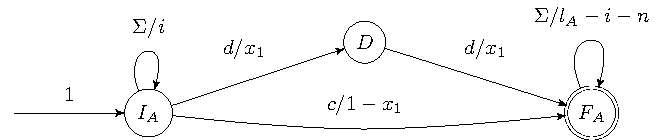
\includegraphics[scale=\autscale]{a_1}
  \caption{ $A'$ with its associated transition variables in symbolic form after
  minimal elminiation of variables using linear algebra. Note the incoming flow
  of $1$ in the starting state and its balancing of the outgoing transitions!
  }\label{fig:a_1}
\end{figure}


As an example, we start with reasoning about $A'$. Performing symbolic reasoning
on these equations and plugging the corresponding symbolic representation of the
constraints on each corresponding integer variable back as an annotation on its
transition, we obtain the automaton in \cref{fig:a_1}. After slightly more
linear algebra to remove variables through equality elimination, we have
\cref{fig:a_2}, whose transitions are only described in terms of the free
variables we care about representing the length of the automaton ($l_A$), the
start of the substring ($i$), and the length of the substring ($n$).

\begin{figure}[h]
  \centering 
  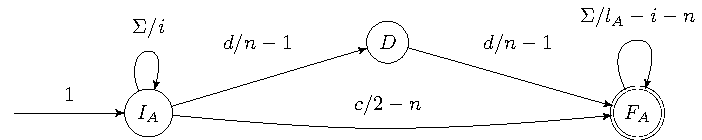
\includegraphics[scale=\autscale]{a_2}
  \caption{ $A'$ after even more linear algebra, with most transitions expressed
  in terms of $n$. Intuitively, this version captures the fact that $n$ is given
  by distributing the incoming flow of $1$ across the two outgoing transitions
  from $I_{A'}$, the initial state.}
  \label{fig:a_2}
\end{figure}

Having obtained this representation, we conclude that $1 < n \leq 2$ from
\cref{const:something-before-and-after,const:something-before-and-after}. The
upper bound is obtained by the following reasoning. Since all transition
variables are nonnegative integers (a transition cannot be used a negative
amount of times), $n \leq 2$ from the $I_A$ to $F_A$ transition. Therefore, it
follows that $n=2$, which implies that the $I_A$ to $F_A$ transition can never
be used under these constraints and that we must use the two $\Char{d}$-labelled
transitions, both now taken $n-1 =1$ times. This immediately implies that the problem is
unsatisfiable, since we know this transition has no correspondance in automaton
$B$.

We repeat similar methods to arrive at the automata in \cref{fig:propagated}.

\begin{figure}[h]
    \centering 
  \begin{subfigure}[b]{0.5\textwidth}
    \centering
    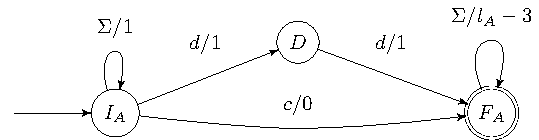
\includegraphics[scale=\autscale]{a_annotated}
    \caption{ $A'$ with its associated transition variables in symbolic
    form.}\label{fig:aut_a_annotated}
      %\Description[SHORT]{LONG}
  \end{subfigure}
  \begin{subfigure}[b]{0.5\textwidth}
    \centering
    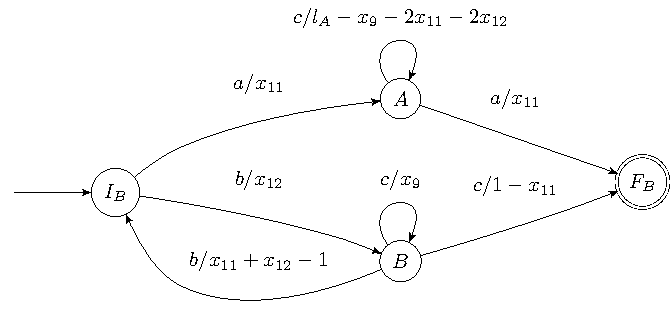
\includegraphics[scale=\autscale]{b_annotated}
    \caption{$B$ with its associated transition variables in symbolic forms.
    Note the large number of implicitly existence-quantified bound variables on
    transitions, suggesting that this automaton has a more complex structure
    with relation to its (free) target variable representing the string length
    than $A'$. The variables used here are fresh, and do not correspond to the
    ones previously used.}\label{fig:aut_b_annotated}
      %\Description[SHORT]{LONG}
  \end{subfigure}
  \caption{The automata after applying linear algebra and equality elimination
  to prune them.}\label{fig:propagated}
\end{figure}


Note that the per-automata length counting registers have been assigned the same
solver variable $l_A$. Since they have to be equal, either one can be used in
both automata through similar applications of equality elimination rules.

At this point we know we have an unsatisfiable solution, \Calculus{} does not.
We press on with concluding that none of the loops of $A'$ at this stage can
become disconnected since they are at the initial and final states, both of
which are trivially reachable for any assignments of the non-constant transition
variables. This means that all valid counter assignments of $A'$ are described
by \cref{eq:counter-sums} and the flow equations alone without the need for
expensive connectivity constraints.

After concluding this, we have a choice of two paths through automaton $B$; the
upper through state $A$ or the lower through state $B$. We case split on a
problem-aware basis by selecting a transition variable that would disconnect
some strongly connected component of automaton $B$, in this case the transition
form $I_B$ to state $B$. We divide it into the cases used ($> 0$) or unused ($ =
0$) since those are the threshold values of the calculus, preferring the latter
option on the first-fail principle.

At this point we have two small, stick-like automata after discounting all
transitions with a corresponding transition variable that is zero, and can try
to compute their product. Doing so, we will immediately notice that the
$\Char{d}$-labelled transition of automaton $A'$ has no correspondence in $B$,
leading to an empty product. We close the proof goal and backtrack with the
opposite constraint, choosing the upper $I_B$ to $A$ transition this time, the
only potentially productive choice we have left. However, proceding with
calculation of the product from the almost identical terms will be similarly
improductive, and we must conclude that the problem is unsatisfiable.

By putting off computing the product $B \times A'$ until after performing linear
reasoning on the number of times each transition must be taken and using that to
prune the terms, we have computed a smaller product than we would have with a
na\"ive approach. Moreover, since this automaton contains only one loop along
one main path, all runs through it can be described by the flow-preservation
equations described above without the need for costly connectivity-enforcing
constraints as in~\cite{generate-parikh-image}.

\section{Preliminaries}\label{sec:preliminaries}
\subsection{Monoids}

% @Philipp: reviewer comment #54 complains that this is basic, are they right?
A monoid $\Monoid = \Tuple{X;\MonoidOp;0_{\Monoid}}$ is an algebraic structure
consisting of the non-empty carrier set of elements, $X$, an associative binary operation
$X \times X \rightarrow X$ denoted as $\MonoidOp$, that is where for all $a, b,
c \in X$, $(a \MonoidOp b) \MonoidOp c = a \MonoidOp (b \MonoidOp c)$. Finally,
$\Monoid$ must have an identity element $0_{\Monoid} \in X$ such that
$0_{\Monoid} \MonoidOp a = a \MonoidOp 0_{\Monoid} =   a$ for every $a \in X$.
We sometimes use integer multiplication to represent repeated application of
$\MonoidOp$, e.g. $3a = a \MonoidOp a \MonoidOp a$, for $a \in X$. $\Monoid$ is
called \textit{commutative} if $\MonoidOp$ also commutes, that is if $a
\MonoidOp b = b \MonoidOp a$ for all $a, b \in X$. 

Finally, a \textit{homomorphism} is a structure-preserving map between two monoids
$\Monoid_1, \Monoid_2$, that is a map $\Map : S_1 \rightarrow S_2$ such that $\Map(a
\MonoidOp_1 b) = \Map(a) \MonoidOp_2 \Map(b)$, where $S_1, S_2$ are the carrier
sets of $\Monoid_1$ and $\Monoid_2$ respectively, and $\MonoidOp_1, \MonoidOp_2$
their binary operations.

\subsection{Languages, Finite-state Automata and their Products}

We define an alphabet as a finite set of symbols $\Alphabet$ with words $\Strings$, and
the concatenation operation as $s_1 \Concat{} s_2$ over two strings $s_1, s_2$.
Note that $\Strings = \Tuple{\Alphabet;\Concat{};\epsilon}$, is a
non-commutative monoid, referred to as the free monoid. The string length
function, $\Length{s}$ is an example of a homomorphism between $\Strings$
and~$\mathbb{Z}$.

An automaton~$\Automaton$ with alphabet~$\Alphabet$ is
$\AutomatonTuple$ where $\Transitions \subseteq \States \times \Alphabet \times
\States$, $\States$ is its states, $\InitialState$ its
initial state, and $\AcceptingStates$ is its set of accepting states.  We
write a transition $\Transition = \Tuple{\State, \Label, \State'} \in
\Transitions$ as $\Transition = \FromLabelTo{\State}{\Label}{\State'}$.
Similarly, we use the notation $\FromLabelTo{\State}{}{}$ to refer to the set of
transitions starting in $\State$, and $\FromLabelTo{}{}{\State}$ to refer to the
set of transitions coming into $\State$, whenever the automaton is clear from
the context.

We will let variables $\Transition, \Transition', \Transition_1, \ldots,
\Transition_n$ etc describe transitions, $\State, \ldots, \State_n$ states, and
$\Automaton, \ldots, \Automaton_n$ automata, and use subscript indexing
($\Transitions_\Automaton$) to refer to the transitions, states, etc of a given
automaton.

By a \emph{product} of two automata $\Automaton_1, \Automaton_2$, written
$\Automaton_1 \times \Automaton_2$, we mean an automaton constructed to run
$\Automaton_1$ and $\Automaton_2$ in parallel on an input and only accept the
input if both automata would do so.

We refer to the resulting product states as tuples, $\Tuple{\State, \State'}$,
which represent the state of the product automaton where $\Automaton_1$ would be
in $\State$ and $\Automaton_2$ would be in $\State'$. Note that since we use
ordered tuples the product is technically (but w.l.o.g) not commutative; the
left-hand-side must come from the left-hand term. The sole purpose of this
matching is to allow us to speak with precision about the origins of components
in a product.

\subsection{The Parikh Map and its Image}
Formally, the \textit{Parikh map} over an alphabet $\Alphabet=
\left\{a_1, \ldots, a_k \right\}$ is defined as in \cite{kozen}:
$$
\begin{aligned}
& \ParikhMap: \MapFromTo{\Strings}{\natural^k} \\
& \ParikhMap(s) = \VectorLiteral{\#a_1(s), \#a_2(s), \ldots, \#a_k(s)}
\end{aligned}
$$

That is, $\ParikhMap(s)$ is a vector of the number of occurrences of each
character in the language for a given string $s$. For example, for  $\Alphabet =
\Set{a, b}$, we would have $\ParikhMap(abb) = \VectorLiteral{1, 2}$.

We define the image of this map, the \textit{Parikh image}, of some subset of
the language $\Language \subseteq \Strings$ as:
\[
\ParikhMap(\Language) = \Set{\ParikhMap(x) \SuchThat x \in \Language}
\]

Thus, we would have $\ParikhMap(\left\{ab, abb\right\}) = \left\{\left[1,
1\right], \left[1, 2\right]\right\}$. We also sometimes use the standard
notation $\#l(w)$ to talk about an individual letter $l$ in a word $w$. For
example, for the Parikh vector above, we would have $\CountOf{a} = 1$.

% @Philipp: Reviewers suggest we drop this:
Parikh's theorem states that any context-free language has a letter-equivalent
regular language (c.f.~\cite{construction} for a construction of such automata
from context-free grammars and~\cite{bounds} for bounds on its size). However,
there are languages that are not context-free that also have semilinear images
under~$\ParikhMap$ (e.g. $\ParikhMap(\Set{a^nb^nc^n \SuchThat n \geq 0}) =
\ParikhMap((abc)^*) = \CountOf{a} = \CountOf{b} = \CountOf{c} \land \CountOf{a}
\geq 0$). This means they can be represented as a quantifier-free Presburger
formula.

Note that while Parikh's theorem applies to context-free languages, in this
paper we focus only on regular languages.

\subsection{The Parikh image of a regular language expressed in Presburger arithmetic}
\label{sec:verma}

Since Parikh images are semilinear, any Parikh image can be written as a set of
linear equations. The version for context-free grammars presented in
\cite{generate-parikh-image} can be straightforwardly adapted for use with a
product of regular languages or Parikh automta. For an intuition, the approach
consists of first computing the product, then assigning each state and
transition an existentially quantified non-negative integer variable, then
describing all paths through the automaton through two sets of equations: one
that preserves the incoming flow across the variables of a state's incoming
transitions is equal to the flow across its outgoing transitions, and one set of
constraints that enforces coherence in the presence of loops by ordering states
by distance in a spanning tree rooted in the initial state.

We refer to this model as the baseline approach, though we also apply
optimisations as described in \cref{sec:implementing-baseline}. The calculus
introduced in this paper, by contrast, lazily enforces the connectedness
constraint while also interleaving the computation of products of automata and
propagating information between the steps to reduce the amount of work that
needs to be done.

\section{Projections on Parikh Images}\label{sec:generalised}
The Parikh map~$\ParikhMap$ represents a homomorphism from the (free)
non-commutative monoid~$\Strings$ to the (free) commutative
monoid~$\Naturals^k$. We are, however, often interested in projections of the
Parikh map, rather than the full image. We therefore consider \emph{arbitrary}
homomorphisms $\Map:\: \Sigma^* \to \Monoid$, where $\Monoid =
\left(X;\MonoidOp;0_{\Monoid}\right)$ is a commutative monoid. We give several
examples of such projections on Parikh images later in this section.

Observe that every homomorphism~$\Map:\: \Sigma^* \to \Monoid$ can be
represented as the composition~$h' \circ \ParikhMap$, for some
homomorphism~$h' : \Naturals^k \to M$. One of the insights underlying our
approach is that it is more efficient to directly compute a
projection on the Parikh image~$\Map(\Language)$, than to first compute the
standard image~$\ParikhMap(\Language)$ followed by projection to
some property of interest.


\begin{example}[String Length]\label{ex:length}
One such simplifying homomorphism can express string
length, the problem that originally motivated our study of the Parikh
map. This mapping is relevant when solving constraints that combine
language membership with string length, for instance the following constraint:
\begin{equation}\label{eq:stringLength}
x \in \Language_1 \wedge y \in \Language_2 \wedge |x| > |y|
\end{equation}

To solve this formula, let
$\Monoid = \Naturals$, and define the homomorphism~$L$ by $L(a) = 1$
for all characters~$a \in \Alphabet$. The length of a string
$s = s_1 \RepeatSum{\Concat} s_n$ is given by
$L(s) = \sum L(s_i) = 1 \RepeatSum{+} 1 = n$, and to solve
\eqref{eq:stringLength} we can instead solve the equi-satisfiable
formula~$\alpha \in L(\Language_1) \wedge \beta \in L(\Language_2)
\wedge \alpha > \beta$. This paper proposes efficient native
procedures to reason about membership constraints
like~$\alpha \in L(\Language_1)$, avoiding the computation of
the complete image~$L(\Language_1)$. This encoding can be seen applied to automaton $B$ in
\cref{ex:string-constraints} (see \cref{fig:aut_b}).
\end{example}

\subsection{Integer Constraints on Strings}\label{sec:parikh-automata}

Parikh images are also applicable for deciding more general classes of string
constraints~\cite{ostrich-plus}. Consider the substring constraint
\cref{const:s1-substring} of \cref{ex:string-constraints}: $ s_1 =
\Substring(s_2, i, n)$, that is $s_1$ is an $n$-length substring of $s_2$
starting at offset $i$ (in some variants , $n$ is $i + |n|$, i.e. the ending
index). That constraint belongs to an expressive fragment of string logic that
cannot be decided by most state-of-the-art string solvers.

In \cref{sec:intuition} we hand-wavily modelled \cref{const:s1-substring} (and
  the other constraints) using \emph{Parikh
  automata}~\cite{parikh-automata,expressiveness}. A Parikh automaton is a
  standard NFA extended such that transitions are additionally labelled both
  with offset vectors defining the increments of a finite number of counters.
  This means that Parikh automata recognise words over an extended
  alphabet~$\Alphabet \times D$, where $D \subseteq \Naturals^d$ is a finite set
  of increment vectors (notation as in~\cite{expressiveness}) and $\Alphabet$ is
  the alphabet of the original NFA.
  
  We use the symbols~$\pi_\Alphabet, \pi_D$ to denote projections to the first
  and the second component of a composite letter~$(a, \Vector{v})$,
  respectively, and extend those projections to words:
\begin{equation*}
  \pi_\Alphabet((a_1, \Vector{v}_1) \RepeatSum{\Concat} (a_k, \Vector{v}_k))
  ~=~ a_1 \RepeatSum{\Concat} a_k,
  \qquad
  \pi_D((a_1, \Vector{v}_1) \RepeatSum{\Concat} (a_k, \Vector{v}_k))
  ~=~ \Vector{v}_1 \RepeatSum{+} \Vector{v}_k.
\end{equation*}

\begin{definition}\label{def:parikh-automata} A Parikh automaton of dimension $d
  \geq 0$ is a pair $\Tuple{\Automaton, C}$, where
  $C \subseteq \Naturals^d$ is a semi-linear set (or, equivalently, a
  Presburger formula), and $\Automaton$ is a finite automaton with the
  alphabet $\Alphabet \times D$, where $D \subseteq \Naturals^d$. We
  say that $\Tuple{\Automaton, \varphi}$ recognises a
  word~$w \in \Alphabet^*$ if and only if the automaton has a run
  accepting an extended word~$w' \in (\Alphabet \times D)^*$ such that
  $\pi_\Alphabet(w') = w$ and $\pi_D(w') \in C$.
\end{definition}

Applied to \cref{const:s1-substring}, the decision procedure in
\cite{ostrich-plus} will construct a pre-image of $s_1$ under the substring
operation, and check whether this pre-image is consistent with the constraint~$s_2 \in \Language(B)$, corresponding to the full product seen in
\cref{ex:string-constraints}. Because the substring operation depends on the
values of the integer variables~$i, n$, a Parikh automaton of dimension~$2$,
shown in \cref{fig:aut_a}, models the pre-image. Intuitively, this construction
accumulates any symbol (for the prefix of the substring operation), incrementing
$i$ to mark the start of the substring, followed by the automaton representing
the substring itself, modified to add a counter to increment $n$ at each
transition, followed by a state that performs no increments and only accepts any
suffix after the matched substring.

% AS: I am quite unsure about which intersection we are looking for here,
% please verify I'm not wrong!
% PR: Sounds right (did some small fixes)
Denoting the language described by \cref{fig:aut_a} as $\Language_{pre}$, we can
then replace $s_1 = \Substring(s_2, i, n)$ and $s_2 \in
\Language(B)$ (of \cref{const:s1-in-c-dd}) with an
equi-satisfiable formula that no longer contains any explicit substring
operation:
%
\begin{equation}
  \label{eq:parikh-constraint}
  p \in \Language_{pre} \wedge~
  \pi_\Alphabet(p) \in \Language(B)
  \wedge~~ \pi_D(p) =
  \begin{bmatrix}
    i \\ n
  \end{bmatrix}~~
  \wedge 0 \leq i \leq i + n \leq |p|
\end{equation}
%
To check the satisfiability of \cref{eq:parikh-constraint}, we need a
decision procedure that can process intersections of regular languages
(in this case, of $\Language_{pre}$ and $\Language(B)$, synchronising
on $\Alphabet$), while imposing the side
condition~$0 \leq n \leq m \leq |p|$ on the increment sum. In
\cite{ostrich-plus}, this decision procedure turned out to be main
bottleneck of the string solver, which was one of the motivations to
develop the lazy algorithm proposed in this paper.

\section{A Calculus for Projections on Parikh Images}\label{sec:calculus}
We start by defining our calculus, \Calculus{}, for one automaton, and only
extend it to products of automata in \cref{sec:multiple}. We assume basic
familiarity with first-order logic, Presburger arithmetic, and the classical
sequent calculus. For reference, see e.g. \cite{Fitting96a}.


First, assume an NFA $\Automaton = \AutomatonTuple$ with $\NrTransitions$
transitions $\Transitions =
\Set{\EllipsisSequence{\Transition}{\NrTransitions}}$. For convenience, we then
introduce the following supporting notations:

\begin{definition}
  A \textit{path} $\Path = \PathEnumeration$ of an automaton~$\Automaton$ with
  transitions $\Transitions$ represents a path through $\Automaton$ using
  transitions in $\Transitions$ (i.e. $\Transitions(\State_k, \Label_{k+1},
  \State_{k+1})$ holds), passing zero or more labels $\Label_1, \ldots,
  \Label_n$. The path must begin in the initial state, i.e.~$\State_0 =
  \InitialState$. The end state, $\State_n$, is not necessarily accepting. If it
  is, we say the path is also \textit{accepting}.
  \end{definition}

\begin{definition}
  Moreover, we talk about the \textit{set of paths} of an automaton,
  $\Paths(\Automaton)$, a possibly infinite (if $\Automaton$ has loops) set of
  valid paths through $\Automaton$. Additionally, we use the
  notation~$\Paths(\Automaton, \State)$ to mean all paths ending in
  state~$\State$.
\end{definition}

\begin{definition}
  For a path $\Path = \Tuple{\State_0 \Label_1 \State_1 \RepeatSum{,}
  \State_n}$, its \textit{word} $\WordOf(\Path) = \Label_1 \RepeatSum{\Concat}
  \Label_n$ is the word read out on its labels.
\end{definition}

\begin{definition}
  The \textit{states} of a path $\Path = \Tuple{\State_0 \Label_1 \State_1
  \RepeatSum{,} \State_n}$, $\StatesOf(\Path) = \Set{\State_0\RepeatSum{,}
  \State_n}$ are the states visited along $\Path$. Note that $\InitialState \in
  \StatesOf(\Path)$ for every path since all paths start in the initial state.
\end{definition}

\begin{definition}
  A \textit{dominating set of transitions}, $C$ of an automaton~$\Automaton$ of
  a transition $\Transition$, written $\Dominates(C, \Automaton, \Transition)$,
  is a set of transitions from $\Automaton$ such that every accepting path $p
  \in \Automaton$ where $\Transition \in p$ contains at least one transition
  from $C$. Notably, $\Dominates(\emptyset, \Automaton, \Transition')$ for every
  dead transition $\Transition'$ and $\Dominates(Set{\Transition''}, \Automaton,
  \Transition)$.
\end{definition}

\begin{definition}
 The \textit{transition count}, $\TransitionCount(\Transition, \Path)$ is the
 number of times a transition $\Transition =
 \FromLabelTo{\State_1}{\Label}{\State_2} \in \Transitions$ appears in a path
 $p$.
\end{definition}

We then introduce the two predicates into our calculus with the following
definitions:

\begin{definition}\label{def:single-image}
  The Parikh predicate, $\SinglePredicateInstance$, for some automaton
  $\Automaton = \AutomatonTuple$, modulo some map $\Map : \Alphabet^* \to \Monoid$ to a
  commutative monoid $\Monoid$ as described in \cref{sec:generalised}
  and with a transition selection function
  $\Filter:\: \Transitions \to \Naturals$ holds when
  $\MonoidElement \in \Monoid$ is an element of the Parikh image of
  $\Language(\Automaton)$
  modulo $\Map$, or more formally when there is an accepting path
  $\Path = \PathEnumeration \in \Accepting{\Paths(\Automaton)}$ such
  that $\Filter(\Transition) = \TransitionCount(\Transition, \Path)$
  for all $t \in \Transitions$, and $\MonoidElement = \Map(\WordOf(\Path))$.
\end{definition}

\begin{definition}\label{def:connected} $\Connected(\Automaton, \Filter)$ for
  some automaton $\Automaton = \AutomatonTuple$ holds when for every
  $\Transition = \FromLabelTo{\State}{}{\State'} \in \Transitions$,
  $\Filter(\Transition) > 0 \implies \exists \Path \in \Paths(\Automaton)$
  $\Filter(\Transition_i) > 0$ for $\Transition_i \in p$, and $\State \in
  \StatesOf(p)$, or in words that there exists some $\Filter$-selected valid
  path that reaches $\Transition$'s starting state, $\State$. It represents the
  condition that $\Automaton$ is connected with respect to the selection
  function $\Filter$ for every transition. It is redundant to $\Image$ by
  design.
\end{definition}

We present the rules of \Calculus{} for one automaton in
\cref{tbl:rules:single}. The rules operate on sets of formulas, and
can be interpreted as rules of a one-sided sequent calculus, in
which all formulas are located in the antecedent~\cite{Fitting96a}.

Each rule should be read and applied bottom-up, and relates
premises~$\SomeClause_1, \ldots, \SomeClause_k$ with some
conclusion~$\SomeClause$. When constructing a proof, we start from some
root~$\SomeClause$, and then apply proof rules to the goals of the proof until a
goal can be closed, or no more rule is applicable.

A proof in which all proof goals could be closed shows that the formulas
in the root~$\SomeClause$ of the proof are inconsistent, and do not
have any solutions. A proof goal that could not be closed, but to which no
more rules are applicable, gives rise to  a solution of the formulas in the
root~$\SomeClause$. Such an open proof goal will only contain formulas
in Presburger arithmetic allowing a solution to be computed using
standard algorithms~\cite{Fitting96a}.

We use the convention of splitting the formulas into linear (in)equalities
($\SomeInequalities$) and other formulas ($\SomeClause$), and assume that
predicates $\Image$ and $\Connected$ only occur positively. Since our rules
operate by adding and matching linear (in)equalities in a proof goal, we use the
shorthand of listing the matched inequalities as antecedents e.g., in
\Propagate{}.

The filtering function~$\Filter$ is evaluated symbolically, and can in practice
be read as a function from transitions to $\Naturals$-valued terms
(e.g.~\texttt{t} or~\texttt{t+1}). In our implementation \Catra{}, described in
\cref{sec:implementation}, $\Filter$~is a vector of fresh variables with the
same size as~$\Transitions$.

We use the shorthand notation~$\Transitions_\Automaton$ to refer to the
transitions of an automaton~$\Automaton$. Additionally, for an
automaton~$\Automaton = \AutomatonTuple$ we allow mapping the selection function
like so: $\Filter(\Automaton) = \Tuple{\States, \InitialState, \AcceptingStates,
\Set{\Transition \in \Transitions \SuchThat \Filter(\Transition) > 0}}$, i.e.
$\Automaton$~with only the transitions for which~$\Filter$ is positive. In this
instance, the basis for the matched linear inequalities is
implicitly~$\SomeInequalities$. Similarly, for our commutative monoid $\Monoid =
\left(X;\MonoidOp;0_{\Monoid}\right)$ and the map into it $\Map : \Strings
\rightarrow X$, we also allow mapping over transitions:
$\Map(\FromLabelTo{\State}{\Label}{\State'}) = \Map(\Label)$.

We require that rules can only be applied when they add new formulas
on every created branch (the notion of \emph{regularity} of a proof is
required~\cite{Fitting96a}). For example, this means that \Split{} can
only be applied to proof goals that contain neither
$\Filter(\Transition) = 0$ nor $\Filter(\Transition) > 0$, and can
never be applied to split on the same term twice on the same branch.
This suggests a proof strategy where you \Propagate{} when you can, \Split{}
when you must, and \Subsume{} when neither is possible anymore.

\begin{table}
\begin{tabular}{@{}l>{$}c<{$}p{3cm}@{}}\toprule
  Name & \text{Rule} & Side conditions\\
  \midrule

  % EXPAND
  \Expand & 
    \inferrule
  {\Connected(\Automaton, \Filter) ,~ \FlowEq(\Automaton, \Filter) ,~ \MonoidElement = \sum_{\Transition \in \Transitions_\Automaton} \Filter(\Transition) \cdot \Map(\Transition), \SomeInequalities, \SomeClause}
  {\SinglePredicateInstance, \SomeInequalities, \SomeClause} & 
  None \\[4ex]

  % SPLIT
  \Split & 
  \inferrule{\Connected(\Automaton, \Filter), \SomeInequalities, \SomeClause, \Filter(\Transition) = 0 \mid \Connected(\Automaton, \Filter), \SomeInequalities, \SomeClause, \Filter(\Transition) > 0}{\Connected(\Automaton, \Filter), \SomeInequalities, \SomeClause} &
  if $\Transition \in \Transitions_\Automaton$ \\[4ex]

  % PROPAGATE
  \Propagate & \inferrule{\Connected(\Automaton, \Filter),
  \Set{\Filter(\Transition') = 0 \SuchThat \Transition' \in C},
  \SomeInequalities, \SomeClause, \Filter(\Transition) =
  0}{\Connected(\Automaton, \Filter), \Set{\Filter(\Transition') = 0 \SuchThat
  \Transition' \in C}, \SomeInequalities, \SomeClause} & if $\Dominates(C,
  \Automaton, \Transition) t \in \Transitions_\Automaton, $ \\[4ex]

  % SUBSUME
  \Subsume &
  \inferrule{\SomeInequalities,\SomeClause}{\Connected(\Automaton, \Filter), \SomeInequalities, \SomeClause} &
  \Split{} and \Propagate{} cannot be applied \\
  \bottomrule
  \end{tabular}
  \caption{Derivation rules for one automaton.}\label{tbl:rules:single}
\end{table}
We use the symbolic function $\FlowEq(\Automaton, \Filter)$ that generates a set
of existentially quantified linear inequalities with the following definition,
where we assign fresh, existentially quantified variables to
$\FinalStateVar_\State, \Filter(\Transition)$ for every $\State \in
\AcceptingStates, \Transition \in \Transitions$:
\[
\begin{aligned}
  \FlowEq(\Automaton, \Filter) &= \sum\limits_{\State \in \AcceptingStates} \FinalStateVar_\State = 1 \land \AndComp{\State \in \States}{\In(\State, \Filter) - \Out(\State, \Filter)} = \Sink(\State) \land
  \AndComp{\State \in \AcceptingStates}{\FinalStateVar_\State \geq 0}\\
  \Sink(\State) & = 0 \text{ if } \State \not\in \AcceptingStates, \FinalStateVar_\State \text{ otherwise.} \\
  \In(\State, \Filter) & = \StartFlow(\State) + \sum_{\Transition \in \FromLabelTo{\State'}{}{\State}} \Filter(\Transition)\\
  \StartFlow(\State)  &= 1 \text{ if } \State = \InitialState, \text{ otherwise $0$.} \\
  \Out(\State, \Filter) &= \sum_{\Transition \in \FromLabelTo{\State}{}{\State'}} \Filter(\Transition)
\end{aligned}
\]

In addition to \cref{tbl:rules:single}, we assume the existence of a rule
\PresburgerClose{}, corresponding to a sound and complete solver for Presburger
formulae, and for the elements of~$\Monoid$.

The $\Propagate{}$ rule allows us to propagate (dis-)connectedness across
$\Automaton$. It states that we are only allowed to use transitions attached to
a reachable state, and is necessary to ensure connectedness in the presence of
cycles in~$\Automaton$.

\textsc{Expand} expands the predicate into its most basic rules; one set of
linear equations synchronising the transitions mentioned by~$\Filter$ to the
corresponding Monoid element~$\MonoidElement$, and the linear flow equations of
the standard Parikh image formulation, as described by~\FlowEq. Since
$\Connected$ and $\Image$ are partially redundant and the difference is covered
by~$\FlowEq$, we can remove the instance of~$\Image$ when applying~$\Expand$. In
this sense, we split the semantics of the $\Image$~predicate into its counting
aspect (covered by $\FlowEq$) and its connectedness aspect (covered by
$\Connected$).

Finally, $\Split{}$ allows us to branch the proof tree by trying to exclude a
contested transition from a potential solution before concluding that it must be
included. Intuitively, this is what guarantees our ability to make forward
progress by eliminating paths through~$\Automaton$.

A decision procedure for our predicate in a tableau-based automated theorem
prover would start by expanding the predicate using the $\Expand{}$~rule. A
theorem prover would perform algebraic substitution on the underlying constants
of~$\Filter$, boiling them down to choices of branches, which depend on one
single variable, and loop transitions. This logic corresponds to the placement
of counters for optimally edge-profiling the CFG of a program, making up a
minimum-spanning tree of the automaton~\cite{path-profiling}.

In order to make the examples below tractable, we will assume the existence of a
rule \EquationReasoning{} that allows us to perform standard algebraic reasoning
on linear inequalities. This rule is not necessary for correctness or
completeness, but shortens the examples considerably.

\subsection{An Example}\label{sec:single:example}
Here we will return to $A'$ from \cref{sec:intuition} and performs the steps of
\cref{sec:intuition:algebra,sec:intuition:prop,sec:intuition:split} with the
formal calculus we just established, but exclude \cref{const:s2-in-b} and
therefore the entire automaton $B$ since we introduce support for products of
automata in \cref{sec:multiple}. Note that this example then becomes
satisfiable, as $s_1 = \Char{dd}, i = 1, s_2 = \Char{adda}, l_A = 4$ is a
satisfying assignment to
\cref{const:more-inside-than-before,const:s1-in-c-dd,const:s1-substring}.

Starting with~$A'$, $\Map$ extracts the increments of a transition (see
\cref{fig:a_1}), $h(\FromLabelTo{q_1}{c / i}{q_2}) = \Vec{v}$ for the increment
vector $\Vec{v}$, concretely $h(\FromLabelTo{I_A}{\Sigma / \left[ l_{A+}, i_+
\right]}{I_A}) = \left[ l_{A+}, i_+ \right]$. We use the same compact notation
here as in \cref{sec:intuition} to represent what is essentially a sparse vector
of $1$ and $0$ coefficients, i.e. = $\left[ l_{A+}, i_+ \right] = \left[1, 1,
0\right]$. Initially, we let $\Filter$ map to fresh variables to obtain:
\begin{equation}\label{eq:single-filter}
    \begin{aligned}
      \Filter(\FromLabelTo{D}{d/\begin{bmatrix}l_{A+}, n_+\end{bmatrix}}{F_A}) & = \TransitionVar_1    & 
                \Filter(\FromLabelTo{F_A}{\Sigma/\begin{bmatrix} l_{A+} \end{bmatrix}}{F_A} ) & = \TransitionVar_2 &       \FlowEq(A', \Filter) & = \begin{aligned}
                    1 + \cancel{\TransitionVar_5} &= \cancel{\TransitionVar_5} + \TransitionVar_3 + \TransitionVar_1\\
                    \TransitionVar_4 &= \TransitionVar_1 \\
                    \TransitionVar_3 + \TransitionVar_1 + \cancel{\TransitionVar_2} &\geq \cancel{\TransitionVar_2}  \\
                  \end{aligned} \\
      \Filter(\FromLabelTo{I_A}{c/\begin{bmatrix}l_{A+}, n_+\end{bmatrix}}{F_A} ) & =  \TransitionVar_3 & 
                \Filter(\FromLabelTo{I_A}{d/\begin{bmatrix}l_{A+}, n_+\end{bmatrix}}{D}) & = \TransitionVar_4 &\\
      \Filter(\FromLabelTo{I_A}{\Sigma/\begin{bmatrix} l_{A+} i_+\end{bmatrix}}{I_A}) & = \TransitionVar_5 & 
    \end{aligned}
\end{equation}

Like in \cref{sec:a_1,sec:intuition:algebra}, we apply reasoning by equivalence
  to end up with fixed values for several of the transition variables
  $\TransitionVar_k$, and eventually we use \cref{const:more-inside-than-before}
  and \cref{const:something-before-and-after} to conclude that the transition
  directly from state $I_{A}$ to $F_{A}$ is incompatible with the constraint.

  Then, following \cref{sec:intuition:subsume}, we remove the $\Connected{}$
   predicate using \Subsume{} since no transition can can become disconnected
   (and in fact never could for $A'$, since all looping transitions are attached
   to the initial and single accepting state and therefore always must be
   reachable from any accepting path). After this, the rest of the reasoning can
   be continued without any part of our calculus, since all values of the
   existentially quantified transition variables
   $\TransitionVar_1,\ldots,\TransitionVar_5$ compatible with
   \cref{const:more-inside-than-before,const:s1-in-c-dd,const:s1-substring,const:something-before-and-after}
   are represented by the flow equations introduced by $\Expand{}$. The
   derivation is shown in \cref{fig:derivation:single}.

\begin{figure}[ht]
  \centering
\begin{prooftree}
  \hypo[]{{\text{Regular solving finishes the proof}}}
  \infer1[]{
    \begin{aligned}
    i = \TransitionVar_5 \land 
    n = 2 \land \\
    2 \geq i \land l_A - i - 2 > 0 
    \land \TransitionVar_2 = l_A - i - 2 
    \land \TransitionVar_3 = 0 \\
    \end{aligned}}
  \infer1[\Subsume: \cref{sec:intuition:subsume}]{
    \begin{aligned}
    \Connected(A', \Filter) \land 
    \TransitionVar_1 = 1 \land 
    i = \TransitionVar_5 \land 
    n = 2 \land 
    2 \geq i \land l_A - i - 2 > 0  \\
    \land \TransitionVar_2 = l_A - i - 2 
    \land \TransitionVar_3 = 0 \\
    \end{aligned}
  }
  \infer1[\EquationReasoning{}: $\TransitionVar_1 = 1$ \cref{sec:a_1}]{
    \begin{aligned}
    \Connected(A', \Filter) \land \\
    i = \TransitionVar_5 \land 
    n = 2\TransitionVar_1 \land n \geq i \land l_A - i - n > 0 
    \land \TransitionVar_2 = l_A - i - n 
    \land \TransitionVar_3 = 1 - \TransitionVar_1 
    \end{aligned}
  }
  \infer1[\EquationReasoning{}: $=$-elimination]{
    \begin{aligned}
    \Connected(A', \Filter)  
    \land i = \TransitionVar_5 
    \land n = \TransitionVar_4 + \TransitionVar_1 
    \land n \geq i 
    \land l_A - i - n > 0 \\
    \land \TransitionVar_4 = \TransitionVar_1 
    \land \TransitionVar_2 = l_A - i - n 
    \land \TransitionVar_3 = 1 - \TransitionVar_1
    \land 1 = \TransitionVar_3 + \TransitionVar_1 
    \land \TransitionVar_4 = \TransitionVar_1 
    \end{aligned}
  }
  \infer1[\EquationReasoning{}: expand $\Sigma, \FlowEq$]{
    \begin{aligned}
    i = \TransitionVar_5 
    \land l_A = \sum_{k = 1}^{k = 5} \TransitionVar_k 
    \land n \geq i \land l_A - i - n > 0
    \land n = \TransitionVar_4 + \TransitionVar_1\\
    \land \Connected(A', \Filter) 
    \land \FlowEq(A', \Filter)
    \end{aligned}
  }
  \infer1[\EquationReasoning{}: expand sum]{
    \Connected(A', \Filter) \land
    \FlowEq(A', \Filter) \land
    \left[l_A, i, n\right] =
    \sum\limits_{\Transition \in \Transitions_{A'} } \Map(\Transition) \cdot \Filter(\Transition)
  }
  \infer1[\Expand{}]{\Image{}_{A', \Map}(\Filter, \left[l_A, i, n\right]) \land n \geq i \land l_A - i - n > 0}
\end{prooftree}
\caption{A derivation tree for an application of
\cref{const:s1-in-c-dd,const:s1-substring,const:something-before-and-after,const:more-inside-than-before}
from \cref{ex:string-constraints}, corresponding to handling the Parikh
automaton $A'$ of \cref{fig:aut_a}. Note the liberal use of removal of equal
variables (e.g. if $x = y$ appears as a statement, we substitute $y$ for $x$
everywhere and drop $\ldots \land x=y \land \ldots$) to keep the size of the
equations managable.}\label{fig:derivation:single}
\end{figure}

To obtain the automaton corresponding to the final model, one can evaluate
$\Filter(\Transition) = k$ for each transition $\Transition$ and construct a
path with each such transition taken $k$ times.

\subsection{Correctness of \Calculus{}}\label{sec:single:correct}

Our correctness proof of \Calculus{} consists of two main parts: we
first show that the construction of a proof always terminates, and
then that each of the proof rules in \cref{tbl:rules:single} is
an equivalence transformation, i.e., does not change the set of
satisfying assignments of a formula. In combination, those two results
immediately imply that \Calculus{} gives rise to a decision procedure.

\subsubsection{\Calculus{} terminates}
\begin{lemma}\label{lma:single-terminates}
  Suppose $\SomeClause{}$ is a set of formulas in which the predicates
  $\Image$ and $\Connected$ only occur positively. There is no
  infinite sequence of proofs~$P_0, P_1, P_2, \ldots$ in which $P_0$
  has $\SomeClause{}$ as root, and each $P_{i+1}$ is derived from
  $P_i$ by applying one of the rules in \cref{tbl:rules:single}.
\end{lemma}

\begin{proof}
  The rule~\Expand{} can only be applied finitely often, since each
  application removes one $\Image$ predicate, and none of the rules
  introduce new instances of the predicate. The rule~\Subsume{} can
  only be applied finitely often, since it strictly decreases the
  combined number of $\Image$ and $\Connected$ predicates in sets of
  formulas, and none of the rules increases that number.

  To show termination of \Split{} and \Propagate{}, observe that the
  $\Filter$ in a predicate~$\Connected(\Automaton, \Filter)$ is never
  updated on a proof branch, which means that the set of terms
  $\Filter(t)$ for $t \in \Automaton$ on every branch is finite. Each
  application of \Split{} and \Propagate{} adds a new
  formula~$\Filter(\Transition) = 0$ or $\Filter(\Transition) > 0$
  to a proof goal, which can only happen finitely often.
\end{proof}

\subsubsection{The rules in \cref{tbl:rules:single} are solution-preserving}

\begin{lemma}\label{lma:single-correct}
  Consider an application of one of the rules in
  \cref{tbl:rules:single}, with
  premises~$\SomeClause_1, \ldots, \SomeClause_k$ and
  conclusion~$\SomeClause$. An assignment~$\beta$ satisfies the
  conclusion~$\SomeClause$ if and only if it satisfies one of the
  premises~$\SomeClause_i$.
\end{lemma}

\begin{proof}
  This property has to be shown by analysing the possible applications
  of each proof rule.

  \Expand{} unfolds the definition of the $\Image$ predicate. To show
  that the rule is solution-preserving we prove the equivalence of the
  upper and lower sets of formulas:
  \begin{itemize}
  \item Assume that $\beta$ satisfies the conclusion, which means that
    there is some accepting path
    $\Path = \PathEnumeration \in \Accepting{\Paths(\Automaton)}$ with
    $\val_\beta(\Filter(\Transition)) = \TransitionCount(\Transition,
    \Path)$ and $\val_\beta(\MonoidElement) =
    \Map(\WordOf(\Path))$. Since immediately implies that $\beta$
    satisfies $\Connected(\Automaton, \Filter)$, since a path is
    connected, and $\FlowEq(\Automaton, \Filter)$ since an accepting
    path satisfies the flow equations. The
    equation~$\MonoidElement = \sum_{\Transition \in
      \Transitions_\Automaton}\Filter(\Transition) \cdot
    \Map(\Transition)$ holds because of
    $\val_\beta(\Filter(\Transition)) = \TransitionCount(\Transition,
    \Path)$.
  \item Assume that $\beta$ satisfies the premise, which implies that
    $\val_\beta(\Filter)$ describes a consistent, connected flow of
    the automaton. By the same argument as in
    \cite{generate-parikh-image}, this flow
    can be mapped to an accepting path~$\Path$ of $\Automaton$ such
    that each transition~$\Transition$ occurs on $\Path$ exactly
    $\val_\beta(\Filter(\Transition))$ times. Together with the equation
    $\val_\beta(\Filter(\Transition)) = \TransitionCount(\Transition,
    \Path)$, this implies that $\beta$ satisfies $\SinglePredicateInstance$.
  \end{itemize}

  In \Split{}, we make use of the fact that $\Filter(\Transition)$ is
  $\Naturals$-valued by definition. For any $\beta$, clearly exactly
  one of $\Filter(\Transition) = 0$ or $\Filter(\Transition) > 0$ will
  be satisfied, implying the property.

  For \Propagate{}, suppose that $\Dominates(C, \Automaton, \Transition)$, which
  means that every accepting path containing~$\Transition$ contains at least one
  of the transitions in $C$. For a $\beta$ satisfying $\Connected(\Automaton,
  \Filter)$. This means that every accepting path $p$ where $\Transition \in p$
  has at least one transition $\Transition' \in C$ such that
  $\Filter(\Transition') = 0$. This means that also
  $\val_\beta(\Filter(\Transition)) = 0$ has to hold since no unbroken path
  containing $\Transition$ exists.

  Finally, for \Subsume{}, observe that if \Split{} cannot be applied,
  then a goal must contain~$\Filter(\Transition) = 0$ or
  $\Filter(\Transition) > 0$ for every $\Transition$. In case the
  formulas in $\SomeInequalities$ are inconsistent, an application of
  \Subsume{} is trivially solution-preserving; therefore assume that
  $\SomeInequalities$ is consistent, which means that it contains
  exactly one of $\Filter(\Transition) = 0$ or
  $\Filter(\Transition) > 0$ for each $\Transition$. Since
  \Propagate{} is not applicable, the transitions~$\Transition$ with
  $\Filter(\Transition) > 0$ must form a connect sub-graph of the
  automaton; this means that $\Connected(\Automaton, \Filter)$ is
  redundant as it is implied by $\SomeInequalities$.
\end{proof}

\section{Parikh Images from Products of Automata}\label{sec:multiple}

We now generalise our calculus to natively work with intersections of
regular languages, or equivalently products of automata. For this
extension, we change the main predicate~$\Image$ to be indexed by a
vector of automata~$\Tuple{\Automaton_1, \ldots, \Automaton_k}$.  For
simplicity, we assume that the sets of states of the $k$ automata (and
therefore also the transition sets) are pairwise disjoint. 
\begin{definition}\label{def:multiple}
  Suppose $\Automaton_1, \ldots, \Automaton_k$ are automata,
  $\Map : \Alphabet^* \to \Monoid$ is a map to a commutative monoid
  $\Monoid$,
  $\Filter: \bigcup_{i=1}^k \Transitions_{\Automaton_i} \to \Naturals$
  is a transition selection function, and
  $\MonoidElement \in \Monoid$. The predicate
  $\ImagePredicate{\Tuple{\Automaton_1, \ldots,
      \Automaton_k}}{\Map}{\Filter}{\MonoidElement}$ is true exactly
  when there are accepting paths~$\Path_1, \ldots, \Path_k$ of the
  respective automata, such that for each $i \in \{1, \ldots, k\}$ and
  $\Transition \in \Transitions_{\Automaton_i}$ it holds that
  \begin{itemize}
  \item the multiplicity of $\Transition$ on $\Path_i$ is consistent with
    $\Filter$, that is,
    $\Filter(\Transition) = \TransitionCount(\Transition, \Path_i)$,
  \item the automata all accept the same
    word~$\WordOf(\Path_i) = \WordOf(\Path_1)$, and
  \item the accepted word is mapped to
    $\MonoidElement = \Map(\WordOf(\Path_i)) =
    \Map(\WordOf(\Path_1))$.
  \end{itemize}
\end{definition}

  \begin{table}[t]
    \begin{tabular}{@{}l>{$}c<{$}p{3cm}@{}}\toprule
      Name & \text{Rule} & Side conditions\\
      \midrule
    
      % EXPAND
      \ExpandM & 
      \inferrule
      {
       {\begin{array}{c}
           \left\{
           \FlowEq(\Automaton_i, \Filter),~~
           \Connected(\Automaton_i, \Filter),~~
           \MonoidElement = \sum_{\Transition \in \Transitions_{\Automaton_i}} \Filter(\Transition) \cdot \Map(\Transition)
           \right\}_{i=1}^k,
           \\[4ex]
          \ImagePredicate{\Tuple{\Automaton_1, \ldots, \Automaton_k}}{\Map}{\Filter}{\MonoidElement}, ~
          \SomeInequalities, \SomeClause
        \end{array}}
        }
      {\ImagePredicate{\Tuple{\Automaton_1, \ldots, \Automaton_k}}{\Map}{\Filter}{\MonoidElement}, \SomeInequalities, \SomeClause} & 
      None \\[5ex]
      \Materialise &
      \inferrule
      {{
         \begin{array}{c}
           \FlowEq(\Automaton', \Filter'),~
           \Connected(\Automaton', \Filter'),~
           \BindingSum(\Automaton_i, \Automaton_j, \Filter')
           \\\ImagePredicate{
                     \Tuple{\Automaton_1, \Automaton_{i-1}, \Automaton_{i+1}, \ldots,
                     \Automaton_{j-1}, \Automaton_{j+1}, \ldots, \Automaton_k,
                     \Automaton'},~ \SomeInequalities, \SomeClause
           }{\Map}{\Filter'}{\MonoidElement}
           \end{array}}
           }
      {\ImagePredicate{\Tuple{\Automaton_1, \ldots, \Automaton_i, \ldots, \Automaton_j, \ldots, \Automaton_k}}{\Map}{\Filter}{\MonoidElement},~ \SomeInequalities, \SomeClause} &
      $\begin{array}{@{}l@{}}
         \Filter' = \Extend(\Automaton_i, \Automaton_j,\Filter),\\
         1 \leq i < j \leq k, \\
      \Automaton' = \Automaton_i \times \Automaton_j,\\
      \end{array}$ \\
      \bottomrule
      \end{tabular}
      \caption{Additional derivation rules for products of arbitrarily many automata.}\label{tbl:rules:multi}
    \end{table}

    For the calculus (\cref{tbl:rules:multi}), we first extend
    $\Expand$ to generate flow equations and instances of $\Connected$
    for each automaton, resulting in a new rule $\ExpandM$.  Unlike
    \Expand{}, \ExpandM{} does not remove the $\Image$~predicate,
    since it is needed to keep track of the currently considered
    partial products.

The rule~$\Materialise$ introduces the product of two individual
automata~$\Automaton_i, \Automaton_j$; this step eliminates
$\Automaton_i, \Automaton_j$ as index of the $\Image$ predicate, and
instead adds the product~$\Automaton_i \times \Automaton_j$, while
also introducing the flow equations and the $\Connected$ predicate.

The rule~$\Materialise$ also has to connect the newly introduced
product~$\Automaton_i \times \Automaton_j$ to the previous automata
$\Automaton_i, \Automaton_j$. This is done by extending the
selection function~$\Filter$ to $\Filter'$, mapping the transitions of the product
to fresh variables~$x_{\Transition}$:
\begin{equation*}
  \Extend(\Automaton_i, \Automaton_j,\sigma)(t)
  ~~=~~
  \begin{cases}
    x_{\Transition} & t \in \Transitions_{\Automaton_i \times \Automaton_j}
    \\
    \Filter(t) & \text{otherwise}
  \end{cases}
\end{equation*}

The multiplicity of transitions in the product then has to be related
to the multiplicities in the individual automata, modelled using the
$\BindingSum$ predicate. The predicate expresses that the multiplicity
of a transition~$\Transition \in \Transitions_{\Automaton_i}$ in
$\Automaton_i$ has to coincide with the sum of the multiplicities of
transitions in $\Automaton_i \times \Automaton_j$ derived from $t$,
and similarly for $\Automaton_j$:
%
  $$
  \BindingSum(\Automaton_i, \Automaton_j, \Filter') ~~=~~
  \begin{aligned}
  & \Set{ 
    \Filter'(\Transition)  =  \sum\limits_{\Transition' = \FromLabelTo{\Tuple{\State, \State_R}}{\Label}{\Tuple{\State', \State_R}}} \Filter'(\Transition')
  \SuchThat \Transition = \FromLabelTo{\State}{\Label}{\State'} \in \Transitions_{\Automaton_i} } \cup\mbox{} \\ 
  & \Set{
    \Filter'(\Transition)  =  \sum\limits_{\Transition' = \FromLabelTo{\Tuple{\State_L, \State}}{\Label}{\Tuple{\State_L, \State'}}} \Filter'(\Transition') \SuchThat \Transition = \FromLabelTo{\State}{\Label}{\State'} \in \Transitions_{\Automaton_j}
  }
  \end{aligned}
$$

\iffalse
Note that this definition implies that $\Filter(\Transition) =
\Filter(\Transition')$ whenever two transitions $\Transition \in
\Transitions_{\Automaton_1}, \Transition' \in \Transitions_{\Automaton_2}$
produces a product transition $\Transition'' \in \Transitions_{\Automaton_1
\times \Automaton_2}$. This corresponds to our intuition that the terms of the
product must agree on the value they accept. As before, we implicitly map
$\Filter$ to fresh terms for each transition in the product.
\fi

For instances of precisely one automaton, neither rule applies and we
perform the calculus as before.

\subsection{An Example}\label{sec:multiple:example}

We return again to our example in \cref{sec:introduction:parikh}, where we
compute the whole Parikh image of the product of $\AcaOrBc{}$ and
$\SomethingCSomething$ under the constraint that there are more instances of
letters a than b. This time our monoid $\Monoid$ is 3-dimensional vectors with
element-wise addition, and $\Map$ that maps each transition to the corresponding
increment vector, e.g $\Map(\FromLabelTo{S}{a}{A}) = \VectorLiteral{1,0,0}$.


In the interest of space, we refer back to
\cref{fig:example:single:equivalences} for the definitions of $\Filter$ for
$\AcaOrBc$ and only define $\Filter$ for $\SomethingCSomething{}$ after
substitutions as follows. Note the expansion of the $\Sigma$ labels:
    \begin{equation*}
      \begin{aligned}
        % & \Filter(\FromLabelTo{S}{a}{A}) & = 1 - \TransitionVar_6 \\
        % & \Filter(\FromLabelTo{S}{b}{B}) & = \TransitionVar_4 + \TransitionVar_6 \\
        % & \Filter(\FromLabelTo{A}{c}{A})  & = \TransitionVar_3  \\
        % & \Filter(\FromLabelTo{B}{b}{S}) & = 2\TransitionVar_6 + \TransitionVar_4 \\
        % & \Filter(\FromLabelTo{A}{a}{F}) & = 1 - \TransitionVar_6 \\
        % & \Filter(\FromLabelTo{B}{c}{F}) & = \TransitionVar_6 \\
        % Other automaton
        \Filter(\FromLabelTo{S}{\Sigma}{S}) & = \VectorLiteral{\TransitionVar_{7a}, \TransitionVar_{7b}, \TransitionVar_{7c}} \\
        \Filter(\FromLabelTo{S}{c}{F}) & = 1 \\
        \Filter(\FromLabelTo{F}{\Sigma}{F}) & = \VectorLiteral{\TransitionVar_{9a}, \TransitionVar_{9b}, \TransitionVar_{9c}} \\
      \end{aligned}
    \end{equation*}
    
In the derivation tree of \cref{fig:derivation:multi} we start as before, but
with the product version of the $\Image$ predicate. The only possible rule here
is $\ExpandM$, which we use to add the corresponding constraints on each
automata of the product as we would have had in the single-automaton version. We
perform algebraic reasoning on those equations, along with the constraint on
$\MonoidElement$ to determine bounds on transition variables that will enable us
to \Subsume{} and remove one of the $\Connected{}$ predicates. When we have
finished doing so, we use \Materialise{} to compute the product of the now
filtered automata. Further algebraic reasoning allows us to remove the final
instance of $\Connected$. We then perform \Expand{} to get rid of the final
$\Image$ instance, and are immediately able to $\Subsume$ the resulting
$\Connected{}$ predicate. This, again, leaves us with a set of linear
inequalities at the leaf that we can use to obtain a model of our final
$\MonoidElement$ values (now a vector). This time we can read out aca, or
$\VectorLiteral{2, 0, 1}$.

\begin{figure}
  \centering
\begin{prooftree}
  \hypo{
    {\begin{array}{lll}
      1 = \TransitionVar_{10} & \land \TransitionVar_3 = \TransitionVar_{11} & \land 1 = \TransitionVar{12} \\ 
      \land 1 = \TransitionVar_{11} &  & \land 2 > 0
    \end{array}}  
  }
  \infer1[\Subsume{}, \Expand{}, \Subsume{}]{
    {\begin{array}{ll}
      2 > 0 \land 1 = \TransitionVar_{10} & \land \TransitionVar_3 = \TransitionVar_{11} \\
      \land 1 = \TransitionVar_{12} & \land 1 = \TransitionVar_{11} \\
      \land \Image{}_{\Automaton', \Map}(\Filter, \VectorLiteral{2, 0, 1}) & \land \Connected(\SomethingCSomething{}, \Filter) \\
    \end{array}}  
  }
  \infer1[\EquationReasoning{}]{
  {  \begin{array}{ll}
      1 = \TransitionVar_{10} \land \TransitionVar_3 = \TransitionVar_{11} & 
      \land 1 = \TransitionVar_{12} \land 1 = \TransitionVar_{11} \\
      \land \Image{}_{\Automaton', \Map}(\Filter, 
      \VectorLiteral{
        \TransitionVar_{7a} + \TransitionVar_{9a},
        0,
        \TransitionVar_{7c} + \TransitionVar_{9c} + 1}) & \land 
        \TransitionVar_6 + \TransitionVar_4 = 0 \\
        \land 1 - \TransitionVar_6 > 0 \land \TransitionVar_6 = 0 &
        \land \TransitionVar_4 = 0 \land  \TransitionVar_3 > 0 \\
        \land 2\TransitionVar_6 + \TransitionVar_4 = 0 & \land 
          \VectorLiteral{
        \TransitionVar_{7a} + \TransitionVar_{9a},
        0,
        \TransitionVar_{7c} + \TransitionVar_{9c} + 1} 
        = \VectorLiteral{
          2,
          0,
          \TransitionVar_3} \\ \land 
      \Connected(\SomethingCSomething{}, \Filter) &
      \land \TransitionVar_{7a} + \TransitionVar_{9a} > 0
    \end{array} } 
  }
  \infer1[\Materialise]{
    {\begin{array}{ll}
      \TransitionVar_6 + \TransitionVar_4 = 0 \land 1 - \TransitionVar_6 > 0 &
      \land \TransitionVar_6 = 0  \land \TransitionVar_4 = 0 \\
      \land \TransitionVar_3 > 0 & \land 2\TransitionVar_6 + \TransitionVar_4 = 0 \\
      \land 
      \VectorLiteral{
        \TransitionVar_{7a} + \TransitionVar_{9a},
        0,
        \TransitionVar_{7c} + \TransitionVar_{9c} + 1}
        = \VectorLiteral{
          2,
          0,
          \TransitionVar_3} & \land
      \Connected(\SomethingCSomething{}, \Filter) \\
      \land 
      \Image{}_{\Tuple{\AcaOrBc{},\SomethingCSomething{}}, \Map}(\Filter, 
      \VectorLiteral{\TransitionVar_{7a} + \TransitionVar_{9a}, 0, \TransitionVar_{7c} + \TransitionVar_{9c} + 1}) & \land \TransitionVar_{7a} + \TransitionVar_{9a} > 0
    \end{array}}
  }
  \infer1[\Subsume{}]{
  {\begin{array}{ll}
    \TransitionVar_6 + \TransitionVar_4 = 0 \land 
    1 - \TransitionVar_6 > 0 &
    \land
    \TransitionVar_6 = 0 \land 
    \TransitionVar_4 = 0 \\
    \land
    \TransitionVar_3 > 0 & \land
    2\TransitionVar_6 + \TransitionVar_4 = 0 \\ 
    \land
    \VectorLiteral{
      \TransitionVar_{7a} + \TransitionVar_{9a},
      0,
      \TransitionVar_{7c} + \TransitionVar_{9c} + 1}
      = \VectorLiteral{
        2,
        0,
        \TransitionVar_3} & \land 
    \Connected(\AcaOrBc{}, \Filter) \\
    \land 
    \Connected(\SomethingCSomething{}, \Filter) \\
    \land 
    \Image{}_{\Tuple{\AcaOrBc{},\SomethingCSomething{}}, \Map}(\Filter, 
    \VectorLiteral{\TransitionVar_{7a} + \TransitionVar_{9a}, 0, \TransitionVar_{7c} + \TransitionVar_{9c} + 1}) & \land \TransitionVar_{7a} + \TransitionVar_{9a} > 0
  \end{array}}
  }
  \infer1[\EquationReasoning]{
    \begin{aligned}
      \VectorLiteral{a, b, c} = \VectorLiteral{
          2 - 2\TransitionVar_6,
          2\TransitionVar_4 + 3\TransitionVar_6,
          \TransitionVar_3 + \TransitionVar_6
        } \land
        \\
        \VectorLiteral{a, b, c} = \VectorLiteral{
            \TransitionVar_{7a} + \TransitionVar_{9a},
            \TransitionVar_{7b} + \TransitionVar_{9b},
            \TransitionVar_{7c} + \TransitionVar_{9c} + 1
          } \land \\
      \Connected(\AcaOrBc{}, \Filter) \land 
      \Connected(\SomethingCSomething{}, \Filter) \land \\
      \Image{}_{\Tuple{\AcaOrBc{},\SomethingCSomething{}}, \Map}(\Filter, 
      \VectorLiteral{a, b, c}) \land a > b
    \end{aligned}
  }
  \infer1[\ExpandM]{\Image{}_{\Tuple{\AcaOrBc{},\SomethingCSomething{}}, \Map}(\Filter, \VectorLiteral{a, b, c}) \land a > b}
\end{prooftree}
\caption{A derivation for \Calculus{} on the Parikh image of strings with more a's than b's in the product of $\AcaOrBc{}$ and $\SomethingCSomething{}$.}\label{fig:derivation:multi}
\end{figure}

\subsection{Correctness of \Calculus{} for Products of Automata}

Since \cref{tbl:rules:multi} only extends the existing rules of
\cref{tbl:rules:single}, we focus on the differences compared
to the calculus for a single automaton.

%\subsubsection{\Calculus{} for products of automata terminates}
\begin{lemma}\label{lma:multi-terminates}
  Suppose $\SomeClause{}$ is a set of formulas in which the product
  version of $\Image$ only occurs positively. There is no
  infinite sequence of proofs~$P_0, P_1, P_2, \ldots$ in which $P_0$
  has $\SomeClause{}$ as root, and each $P_{i+1}$ is derived from
  $P_i$ by applying one of the rules in \cref{tbl:rules:multi}.
\end{lemma}

\begin{proof}
  The rule \Materialise{} can similarly only be used finitely many times, as
  each application reduces the number of automata in the product of $\Image$ by
  one automaton, until only one remains and \cref{lma:single-terminates} for
  single-automaton instances applies.
  
  This implies that also the rule~\ExpandM{} can only be applied
  finitely often since its side condition only allows applying it once
  per instance of an $\Image$ predicate containing a product, and only finitely
  many instances of $\Image$ can be introduced on each branch.
\end{proof}

%\subsubsection{The rules in \cref{tbl:rules:multi} are solution-preserving}

Since our calculus now includes a rule introducing new variables, the
\Materialise{} rule, we have to slightly generalise the notion of
solution-preservation:
%
\begin{lemma}\label{lma:multi-correct}
  Consider an application of one of the rules in
  \cref{tbl:rules:multi}, with
  premises~$\SomeClause_1, \ldots, \SomeClause_k$ and
  conclusion~$\SomeClause$. An assignment~$\beta$ (over the symbols in
  $\SomeClause$) satisfies the conclusion~$\SomeClause$ if and only if
  there is an extension~$\beta' of \beta$ satisfying one of the
  premises~$\SomeClause_i$.
\end{lemma}

\begin{proof}
  We have to consider the two new rules in \cref{tbl:rules:multi}. The
  result is immediate for \ExpandM{}, since this rule does not remove the
  $\Image$ predicate from a proof goal, and the newly introduced formulas
  are all implied by the $\Image$ predicate.

  For \Materialise{}, observe that the existence of an accepting path
  in $\Automaton_i \times \Automaton_j$ is equivalent to the existence
  of individual paths in $\Automaton_i, \Automaton_j$ accepting the
  same word. The path in the product will satisfy the flow equations
  and connectedness, and it will be related to the individual paths as
  stipulated by the \BindingSum{} predicate.
\end{proof}


\section{Extensions}\label{sec:extensions}

This section describes a number of possible extensions to the calculus. Note
that some are partially or fully implemented in \Catra{} already. In particular,
we have some level of support for symbolic transitions over Unicode alphabets to
keep practical automata under a reasonable size, though we do not allow a full Boolean algebra over symbols as described e.g. in~\cite{symbolic-automata}.

\subsection{Backjumping and Learning No-Goods}\label{sec:ext:backjumping}

\Calculus{} can be accelerated for some instances by adding rules for
backjumping. In particular, key connectedness constraints for an automaton can
be learnt. In that case, when discovering that a transition $\Transition$ of an
automaton $\Automaton$ under a certain transition variable $\Filter$ has become
unreachable, we can learn the clause $\Connected(\Automaton, \Filter) \land
\sum_{\Transition' \in C} \Filter(\Transition') = 0 \implies \Transition = 0$ where
$\Dominates(C, \Automaton, \Transition)$ for some minimal $C$. Note that this
captures both forward (unrachable from the initial state) and
backward (does not reach an accepting state) unreachability. Bidirectional cut
learning is implemented in \Catra, and has provided a slight improvement in
performance on some instances.

The other source of clauses to learn is the \Materialise{} rule. Whenever an
attempt to materialise a product of two ($\Filter$-filtered) automata
$\Automaton_1 \times \Automaton_2$ produces an empty product, we can determine
the cause of the failure with respect to the automata and their respective
transition variables, and learn no-good combinations that can never be part of a
model. In order to be able to do this, we need a few semantic predicates to
record the state of the calculation, as well as a system of disambiguating
automata, since it is possible to arrive at the same automaton by multiple
combinations of decisions and products. In \Catra{}, we use a number of
additional predicates to record the status of the materialisation of products,
to separate instances of our main predicate, and to register the mapping between
automata and their respective transition $\Filter$ terms, described in
\cref{sec:implementation}. However, at this point only rudimentary no-good
learning is implemented.

\subsection{Symbolic Automata}\label{sec:ext:symbolic}

Extending \Calculus{} to support fully symbolic automata is possible within the
framework, depending on your choice of $\Map$. The difficulty consists in
handling the mapping of the homomorphism $\Map$ over symbolic labels, assuming
it maps to finitely many monoid elements. This is not always straightforward, as
seen in the example of \cref{sec:multiple:example}. This complexity is inherent
in computing the full Parikh image, and stems from the fact that we need to
differentiate between the possible interpretations of the $\Sigma$ transitions
without knowing ahead of times which ones will actually be materialised in the
product. If, on the other hand, if our $\Map$ had been length-counting, which
does not differentiate between values, it would have required no adaptation at
all. With a somewhat liberal interpretation of what we are allowed to map to
(e.g. fresh terms), it is possible to use $\Map$ to represent choice operations
like the ones in a range label. In \Catra{}, we frontload this problem by
requiring the user to encode their input as a Parikh automaton. For an example of how automata can be encoded, see \cref{sec:parikh-automata}.

\subsection{Transducers}\label{sec:ext:transducers}

Another interesting application is applying \Calculus{} to automata with
multiple tracks, e.g. transducers. One application of such a calculus would be
to represent replace operations and other functions on regular languages, and to
be able to answer questions like "does this operation change the length of the
string". The difficulty in implementing it for transducers is first to perform
the mapping on the labels, which for both the length and Parikh cases is
straightforward; just do the same thing in two dimensions. The more complicated
operation is defining the product of transducers. In some cases it would
probably be desirable to perform synchronisation (e.g. requiring overlapping
transitions) on only some transitions, for example the first track.

Implementing such a calculus is straightforward in \Calculus, since the
definition of products was left out of the definition. All that would be needed
is an appropriate update of the definitions of products. Simiarly, \Catra was
written with modularity in mind, and it should be straightforward to extend both
the input grammar and automata implementations to accommodate multi-track
automata with arbitrary synchronisation.

\subsection{Finding the Presburger representation of a homomorphic image}\label{sec:finding-the-image}

To find the Presburger form of the homomorphic image efficiently, we adapt the
quantifier elimination approach of~\cite{qe} to our problem domain. The core
method is the same: we incrementally use \Calculus{} to find models,
\Generalise{} the models we find into a quantifier-free Presburger formula with
the $\MonoidElement$ as the only free variable (algorithm~\ref{alg:generalise}), add the
negated formula as a constraint, and continue enumerating models until none
remain. The disjunction of the generalised models we enumerated is now our
image.

\begin{algorithm}
  \caption{$\Generalise{}(\Automaton, \Filter, a)$ will generalise a final product $\Automaton$ and a model $a$ under the homomorphism $\Map$.}\label{alg:generalise}
  \KwData{$\Automaton$, a product from \Calculus{}, a model $a$ assigning counts to the terms that $\Filter$ associate with each transition of $\Automaton$, and our homomorphism $\Map$ that we want to compute the image modulo.}
  \KwResult{a quantifier-free Presburger formula $P$ representing a partial $\Map$-homomorphic image}
  \SetKwFunction{EliminateQuantifiers}{eliminateQuantifiers}

  $\Automaton' \gets \Tuple{\Automaton_\States, \Automaton_{\InitialState}, \Automaton_\AcceptingStates, \Set{\Transition \in \Automaton_\Transitions \SuchThat a(\Filter(\Transition)) \neq 0}}$

  \KwRet{\EliminateQuantifiers{$\Map(\ParikhMap(\Automaton'))$}}
  \end{algorithm}


  \begin{algorithm}
    \DontPrintSemicolon
    \caption{$\FindImage{}(\Automaton_1 \times \ldots \times \Automaton_k, \Map)$ will find the Presburger form for the product $\Automaton_1 \times \ldots \times \Automaton_k$ modulo a homomorphism $\Map$ where the only free variable is/are the one(s) representing the monoid element of $\Map$.}\label{alg:find-image}
    \KwData{$\Automaton$, a product from \Calculus{}, a model $a$ assigning counts to the terms that $\Filter$ associate with each transition of $\Automaton$, and our homomorphism $\Map$ that we want to compute the image modulo.}
    \KwResult{a quantifier-free Presburger formula $P$ representing a partial $\Map$-homomorphic image}
    \SetKwFunction{NewTheoremProver}{newTheoremProver}
    \SetKwFunction{EliminateQuantifiers}{eliminateQuantifiers}
    \SetKwFunction{FreshVariable}{freshVariable}
    \SetKwFunction{Assert}{assert}
    \SetKwFunction{GetModel}{getModel}
    \SetKwData{ImageVar}{image}
  
$p \gets \NewTheoremProver{}$\;
$\Filter(\Transition) := \FreshVariable{p}$ for every $\Transition \in \Transitions_{\Automaton}$\;
$\MonoidElement \gets$ \FreshVariable{$p$}\;
\Assert{$p, \exists \MonoidElement, \Filter(\Transition) \text{ for every } \Transition \in \Transitions_\Automaton \HoldsThat \ImagePredicate{\Automaton}{\Map}{\Filter}{\MonoidElement} \land \AndComp{\Transition \in \Transitions}{\Filter(\Transition) \geq 0}$}\;
$\ImageVar \gets \bot$\;
\While{$p$ has more models}{
  $\Tuple{\Automaton, a} \gets \GetModel(p)$\;
  $G \gets \Generalise{}(\Automaton, \Filter, a)$\;
  $\ImageVar \gets G \lor \Image$\;
  \Assert{$p, \lnot G$}\;
  }
    \KwRet{\ImageVar}
    \end{algorithm}

    The \GetModel{} function is nonstandard in that it returns both the model
    and its associated automaton. Since algorithm~\ref{alg:find-image} is
    essentially a form of quantifier elimination and therefore an internal affair
    to the theorem prover, this should be considered fair game.
    
    A preliminary implementation of this approach is available as part
    of~\Catra, but has been neither optimised nor fully tested.


\section{Implementation}\label{sec:implementation}

We implement \Calculus{} for Parikh automata as described in
\cref{sec:parikh-automata}. The artefact submitted along with this paper is a
program that reads an instance file with one or more products of one or more
Parikh automaton with transition labels defined as ranges of Unicode characters,
along with a set of constraints on the final values of their registers expressed
as Presburger arithmetic in a C-like syntax. We call this program
\Catra.
% \footnote{If you really must read it as an acronym, please read it as
%CAtegory Theory on Register Automata, or if you object to the somewhat
%nonstandard use of register automata and category theory, as Check Assignments
%of The Registers Afterwards. Or alternatively if you find it all to be too much
%of a theoretical exercise, as Can Anyone Think of A Real Application.}

\Catra{} is written in Scala, with the calculus described in this paper
implemented as a theory plug-in for the \Princess{} automated theorem
prover~\cite{princess}, which also performs the Presburger reasoning. For
comparison, we also provide an implementation of the baseline method
from~\cite{generate-parikh-image}, a direct translation that uses the~\Nuxmv{}
symbolic model checker~\cite{nuxmv} to solve our constraints, and the
approximation described in~\cite{approximate-parikh} on top of the standard
baseline back-end. An example of an input file corresponding to our running
example introduced in \cref{sec:motivation} can be seen in
\cref{lst:input-example}.

\Catra{} uses symbolic labels for automata. A symbolic label is defined as a
finite range of Unicode code points. This allows succinct representation of many
regular expression patterns such as \lstinline{(a-z).*} which would have
otherwise required $27$~transitions. The transition for the range would be
written \lstinline{a -> b [97, 122]}.

In satisfaction mode, supported by all backends, \Catra{} tries to satisfy the
constraints expressed by the input file, reporting \Sat{} with register
assignments or \Unsat{} much like traditional~SAT- or SMT solvers would.
Additionally, baseline and \Calculus{} also support generation of the Presburger
formula describing the constraints of the input file. Baseline uses standard
quantifier elimination, and \Calculus{} uses the method described in
\cref{sec:finding-the-image}.

Since \Princess{} does not support multiple-arity predicates like the ones we
use in \Calculus{}, we have implemented variable-length arguments using
additional helper predicates. These are $\Unused{}(\Automaton)$, which marks an
automaton as unused in any product, and $\TransitionMask{}(\Automaton,
\Transition, \Filter(\Transition))$ which associates a transition $\Transition$
and automaton $\Automaton$ with its corresponding transition variable.
Additionally, we associate each of our predicates with an instance variable in
order to differentiate instances of the predicates.

\subsection{Implementing the Baseline}\label{sec:implementing-baseline}

We baseline using the same Presburger solver (\Princess{}), input file parser,
and automaton implementation as \Catra. We do this in order to better analyse
the impact of the calculus rules themselves. Using the formula of
\eqref{eq:generate-parikh}, we produce quantified Presburger formulae for each
successive term and add them to \Princess. We compute the product incrementally
term by term, checking satisfiability at each step. We use a priority queue to
select automata for each step, and order it by the number of transitions as a
heuristic for the size of the automata. We use this heuristic to avoid computing
large (and therefore slow) products until we have to, banking our hopes on
computing an empty intermittent product early.

\begin{algorithm}
  \caption{How we implement the baseline approach}\label{alg:baseline}
  \KwData{$\Automaton_1, \ldots, \Automaton_n$ automata, other constraints $\SomeClause$}
  \KwResult{\textsc{Sat} or \textsc{Unsat}}
  \SetKwFunction{NewTheoremProver}{newTheoremProver}
  \SetKwFunction{NewPriorityQueue}{newPriorityQueue}
  \SetKwFunction{Dequeue}{dequeue}
  \SetKwFunction{Enqueue}{enqueue}
  \SetKwFunction{Assert}{assert}

  $p \gets \NewTheoremProver{}$

  \Assert{$p$, $\SomeClause$}

  \ForEach{$\Automaton_i$}{
    \Assert{$p, \ParikhMap(\Automaton_i)$}

    \If{$p$ is \textsc{Unsat}}{break}

  }

  $q \gets \NewPriorityQueue{}$


  \While{$p$ not \textsc{Unsat} and $|q| > 1$}{
    $\Automaton, \Automaton' \gets \Dequeue{q}$ 
    
    \Assert{$p, \ParikhMap(\Automaton \times \Automaton')$}

    \Enqueue{$q, \Automaton \times \Automaton'$}
  }
  
  \KwRet{$p$'s SAT status}

  \end{algorithm}

As an optimisation, our automata (including intermittent products) are created
forward- and backward- reachable-minimal. Any automaton we produce only contains
states that are both reachable from the initial state and has a path to an
accepting state. We never perform any other minimisation on the automata for
either backend. More complex minimisation was left out since performing
minimisation on automata with counters is non-trivial, and minimising symbolic
automata risks exponential blowup \cite{minimising-symbolic}.

\subsection{Heuristics and search strategies}

There are a number of choices left unspecified in \Calculus{} as described in
\cref{sec:calculus,sec:multiple}. For example, the order of materialisation of
intermediate products and the order of splitting. In this section we describe
additional implementation details and techniques used to enhance \Catra.

\subsubsection{Splitting, Materialisation, and Propagation}

We order our rule applications so that we first propagate connectedness if
possible, then perform materialisation if tractable as defined below, then
finally resort to splitting if we must.

In addition to applying \Split{} as described in \cref{tbl:rules:single} to
randomly selected transitions, we prefer splitting to sever a strongly connected
from the initial state. We randomly select an automaton where we can compute a
cut between an SCC and the initial state, that is where the SCC does not contain
the initial state and where the sum of the transition variables of the
transitions in the cut is not known to be positive. If there are multiple such
strongly connected components we choose one randomly. We then proceed to split
on the sum of the transition variables of the cut as if it were a regular
transition, e.g. its sum being zero or nonzero. In this way we drive \Calculus{}
towards applying \Propagate{}.

The implementation of the connectedness constraint is opportunistic and straightforward. We compute a set of dead states by performing forward and backwards reachability computations on an automaton, where we disregard any transition whose associated variable is known to be zero. After that we add clauses ensuring any transition variable associated with a transition starting in a dead state is zero.

Product materialisation is the final piece of the puzzle. In the current
implementation we put off computing intermediate products until at least all but
two transition variables of one of the automata is known to be either present or
absent. The number was chosen experimentally, and we observe a consistent trend
towards lower numbers being better. The other automaton for the product is
selected randomly.

\subsubsection{Clause Learning}

\Catra{} enables clause learning by default when using our backend, as it has
been experimentally shown to increase the performance in aggregate (though not
strictly). We do not currently implement all the proposed features of
\cref{sec:ext:backjumping}, but we do implement forward-reachability cut
learning. No sophisticated clause learning for products has been implemented.

\subsubsection{Random Restarts}

Finally, we perform restarts scaled by the Luby series~\cite{luby}. Experimental
results have shown this to have a large improvement in performance, which is
unsurprising given how many random choices we make during solving and how
tail-heavy our problem is.

\section{Evaluation}\label{sec:experiments}

We evaluate the performance of \Catra{} on~\NrBenchmarks{} instances of Parikh
automata intersection problems generated by the \OstrichPlus{} string constraint
solver~\cite{ostrich-plus} when solving the PyEx benchmarks, 
which are string constraints from symbolic execution that are known
to be hard for many solvers~\cite{pyex}. After generating an
initial~\InitialNrBenchmarks{}, we remove~\NrTrivial{} instances solved in under
five seconds by baseline as well as~\NrInvalid{} instances that were duplicates of other instances in the set.

 We also attempted to benchmark instances generated by
\OstrichPlus{} solving the Kaluza benchmarks~\cite{Saxena10:kaluza}
(\numprint{38227}~instances),
\iffalse
and pyex-len
(\numprint{791}~instances) benchmark suites\fi
but discarded them since they all turned out to be trivial for our tool
\Catra{}: every instance
could be solved in under five seconds, with a mean runtime of about 0.1s.
The benchmarks are run
on commit~\texttt{\commit} of \Catra{}\footnote{Github repository redacted for anonymity.}.

The benchmarks are executed in parallel across a cluster of identical
machines, \BenchmarkRig{}, as the sole job for each machine.  We compiled
the code using Scala~\ScalaVersion{} and executed the experiments
on~\JvmVersion{} with a maximum heap of~\MaxHeapSize{}. We used \Nuxmv{}
version~\NuxmvVersion{} invoked as a subprocess for each instance. Instances
were executed in batches of \BatchSize{}, each given a fresh JVM. Each JVM was
warmed up for \numprint{10}s on a random benchmark from the set before starting
to execute. We believe this represents a realistic use case where \Calculus{} is
used to support, e.g., a string solver. Experiments were executed in random order
for all backends. Each instance got a time budget of~\RuntimeTimeout{}.

All runtimes are measured in wall-clock time as observed by the JVM when
executing the instance, and exclude time spent parsing (usually far below
\numprint{0.1}s).

\subsection{Execution Time and Ability to Solve Instances}\label{sec:runtime}

\begin{figure}[t]
  \centering
  \begin{subfigure}[b]{0.49\textwidth}
    \includegraphics[width=\textwidth]{graphs/\commit-by-solver.pdf}
    \caption{The division of statuses per backend.}
    \label{fig:solve-division}
    \Description[A bar chart showing three bars, one per backend, illustrating how many instances they could solve]{The bars are divided by satisfiable and unsatisfiable instances. Baseline could seemingly only solve unsatisfiable instances, PC* could solve a few satisfiable and mostly unsatisfiable, and nuxmv could solve about twice as many unsatisfiable as satisfiable instances, and slightly less in total than PC*.}
  \end{subfigure}
  \hfill
  \begin{subfigure}[b]{0.49\textwidth}
    \includegraphics[width=\textwidth]{graphs/\commit-time-boxplot.pdf}
    \caption{The distribution of runtimes for solved instances per backend, assuming they were solved within the \numprint{30}s timeout.
    The whiskers use the default placement in Pandas, \numprint{1.5} times the IQR (interquartile range).}
    \label{fig:runtime-boxplot}
    \Description[A box plot showing the distribution of runtime over the three backends]{The middle box plot shows a tiny box centered around 0 seconds for the PC* backend, the rightmost box shows a bigger box between five seconds and 30 seconds for nuxmv, and the leftmost box shows a smaller box between 20 and 30 seconds for baseline. The whiskers of nuxmv span between 0 and the timeout, 60 seconds, while they are much tighter for PC*. On the other hand, PC* has a lot of outliers.}
  \end{subfigure}
  \vfill
  \begin{subfigure}[b]{\textwidth}
    \includegraphics[width=\textwidth]{graphs/\commit-cactus.pdf}
    \caption{The number of instances solved as the time budget increases, simulated from one \numprint{120}s-timeout run.}
    \label{fig:cactus}
    \Description[A cactus plot comparing the performance of nuxmv, PC* and baseline]{The line for baseline is strictly lower than the two others, and does not head upwards from zero until after 10 seconds of timeout, while the number of instances for nuxmv increases sharply until ca 10 seconds and then linearly after that. Lazy solves much more instances than nuxmv.}
  \end{subfigure}
  \caption{Evaluation of \Calculus{} solving Parikh automata problems generated by \Ostrich{}.}
\end{figure}


In \cref{fig:solve-division}, we show how many of the~\NrBenchmarks{} instances
the respective back-end could solve. A summary of their outcomes by instance
type is also available in \cref{tab:solve-status}. Note that many instances lack
a ground truth as they are solved by only one backend. We see that
\Calculus{} generally outperforms \Nuxmv{} on determining unsatisfiability, as
does baseline, while being similar at satisfiable instances. Both \Calculus{} and
\Nuxmv{} outperforms baseline on satisfiable instances. On satisfiable
instances, \Nuxmv{} and \Calculus{} have similar performance.

Baseline performs worse on satisfiable instances because it executes a heuristic
meant to detect unsatisfiability early, similar to~\cite{approximate-parikh}.
The heuristic is enabled since the improvement is significant compared to the
extra cost.

\begin{figure}[t]
  \centering
  \begin{subfigure}[b]{0.49\textwidth}
    \includegraphics[width=\textwidth]{graphs/\commit-duels-lazy-baseline-scatter.pdf}
    \caption{Per-instance runtime between baseline and \Calculus{}}
    \label{fig:duels:baseline}
    \Description[A scatter plot showing individual instances as dots compared to \Calculus{} and baseline]{The plot shows most dots at the bottom of the plot, with some plots collected at the right-hand side.}
  \end{subfigure}
  \hfill
  \begin{subfigure}[b]{0.49\textwidth}
    \includegraphics[width=\textwidth]{graphs/\commit-duels-lazy-nuxmv-scatter.pdf}
    \caption{Per-instance runtime between \Nuxmv{} and \Calculus{}}
    \label{fig:duels:nuxmv}
    \Description[A scatter plot showing individual instances as dots compared to \Calculus{} and \Nuxmv{}]{The plot shows flames of dots between the bottom and top, with a line of dots near the right-hand side corresponding to timeouts.}
  \end{subfigure}
\end{figure}


Finally, in \cref{fig:runtime-boxplot,fig:duels:baseline,fig:duels:nuxmv} and we compare
runtimes for solved instances between the backends. We see that \Nuxmv{} has a more even spread of runtimes up to \numprint{20}s,
while both \Calculus{} and baseline tend towards solving their
instances quickly or not at all, though \Calculus{} does have a long tail of outlier
instances that finish as the timeout increaseses.
Notably, \cref{fig:duels:baseline} shows that any instance solved by baseline in \numprint{30}s is also
solved by \Calculus{} in under \numprint{5}s.

\begin{table}
  \begin{center}
  \begin{tabular}{lrrr}
\toprule
backend & baseline & \Calculus & \Nuxmv \\
status after $30$s &  &  &  \\
\midrule
\textsc{Sat} & 6 & 3692 & 3288 \\
\textsc{Unsat} & 8958 & 15197 & 6356 \\
\bottomrule
\end{tabular}

  \end{center}
  \caption{Number of successful results within a timeout of \RuntimeTimeout{}.
  Instances solved by no backend within the timeout (about half of the set) are
  omitted from the table.}\label{tab:solve-status}
\end{table}

\subsubsection{Scalability}\label{sec:scaling}%
To investigate scaling we additionally execute \numprint{2000} randomly sampled
(without replacement) benchmarks with a \numprint{120}-second timeout. We add
runs of \Calculus{} with clause learning and restarts disabled, and with only
clause learning disabled to show the impact of \cref{sec:random-restarts}, and
\cref{sec:clause-learning} respectively.

A cactus plot showing the number of instances solved within a given timeout can
be seen in \cref{fig:cactus}. We see that \Calculus{} outperforms \Nuxmv{} in
general but that \Nuxmv{} might scale better on very long runtimes. This is
likely due to two factors. First, \Nuxmv{} is more mature than \Calculus{}, and
its more general model checking methods might pay off on more difficult
instances compared to problem-specific methods. Second, for longer-running
calculations clause learning as described in \cref{sec:clause-learning} might
matter more. As clause learning in \Catra{} is rudimentary and generalises
poorly across product computations, there is a performance hit.

\subsection{Evaluation in \Ostrich{}}\label{}%

\begin{table}
  \begin{center}
  \begin{tabular}{lrrrrrrr}
\toprule
solver & CA-Str & Competitors & \Ostrich{} 1.3 & \Ostrich{}+CA & Z3-Noodler & cvc5 & z3alpha \\
kind &  &  &  &  &  &  &  \\
\midrule
\textsc{Sat} & 6427 & 14207 & 9586 & 9930 & 7344 & 14069 & 13599 \\
\textsc{Unsat} & 5562 & 7574 & 7356 & 7387 & 5367 & 7377 & 7298 \\
\bottomrule
\end{tabular}

  \end{center}
  \caption{Number of solved benchmarks in the set of quantifier-free strings with
    linear integer arithmetic constraints (QF\_SLIA) at SMT-COMP~2023. The numbers are from
    the competition results, except for CA-Str, which is executed by us on the same 
    cluster as the competition with the same resources, and the two virtual portfolio solvers
    \Ostrich+CA and \textsc{Competition} which aggregate the best results from \Ostrich{}/CA-Str and 
    all the competition results for non-\Ostrich{} solvers respectively. }
  \label{tab:solve-status-smt-comp}
\end{table}

\begin{figure}[t]
  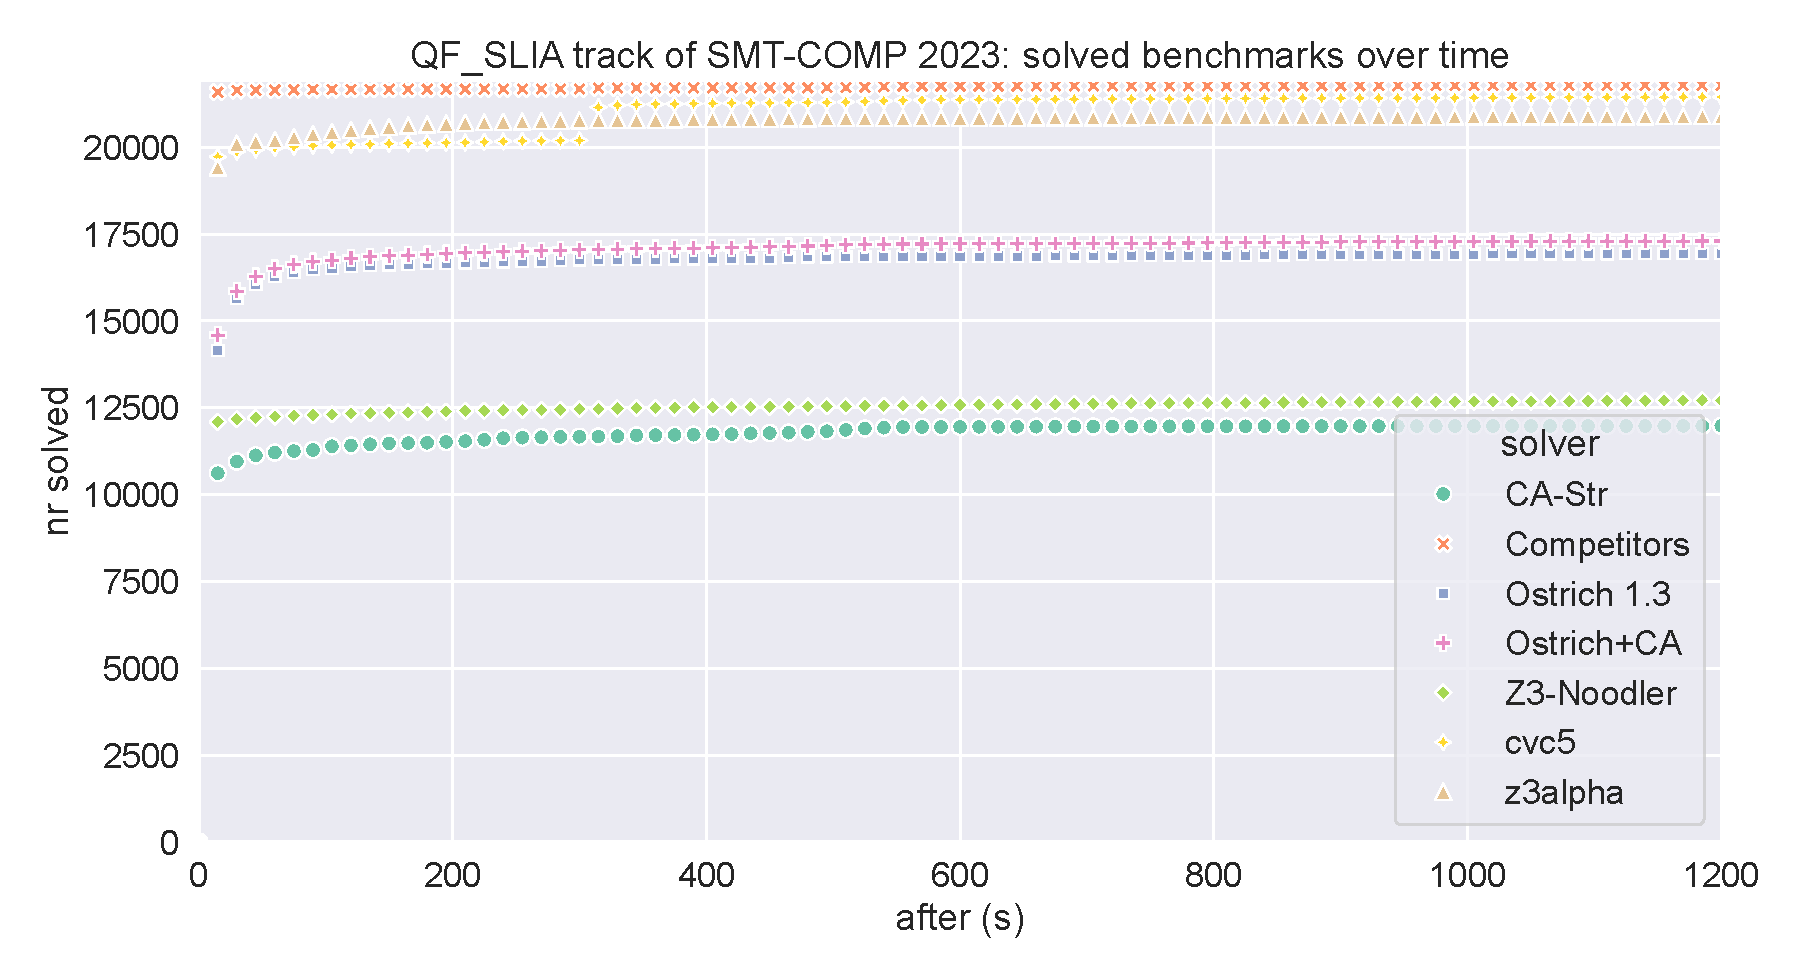
\includegraphics[width=\linewidth]{graphs/smt-comp-cactus}
  \caption{The number of instances solved in the QF\_SLIA track of SMT-COMP 2023
   as the time budget increases towards the competition limit of \numprint{20}~minutes.}
  \label{fig:smt-comp:cactus}
  \Description[A cactus plot comparing the performance of the solvers in the QF_SLIA track of SMT-COMP]%
  {The plot shows the results for the solvers Ostrich 1.3, CA-Str, Ostrich+CA, Z3-Noodler,
  cvc5 and z3alpha as number of solved instances (y-axis) after N seconds (x-axis). The
  topmost solver is the virtual portfolio "Competition", representing every non-Ostrich
  solver, followed by cvc5, after ca 200 seconds, after which it overtakes the previous leader, z3alpha.}
\end{figure}

To evaluate the effectiveness of \Calculus{} in a string solver, \Catra{} was
experimentally integrated as the Parikh automata product solver into the string
solver \Ostrich{}~version~1.3. \Ostrich{} is an independently developed solver
that participated in the recent
SMT-COMP~2023\footnote{\url{https://smt-comp.github.io/2023/participants/ostrich}},
winning the single-query track for quantifier-free strings (\texttt{QF\_S}), as
well as dominating other solvers on unsatisfiable string
benchmarks~\cite{smt-comp-23}.

 At SMT-COMP, \Ostrich{} competed using a portfolio of three different
 back-ends:
\begin{itemize}
\item \textbf{BW-Str:} a backward-propagation-based solver, not utilising
  Parikh automata~\cite{ostrich}.
\item \textbf{ADT-Str:} a solver based on algebraic data-types.
\item \textbf{CE-Str:} a re-implementation of the \OstrichPlus{}
  algorithm~\cite{ostrich-plus}, using Parikh automata and the
  encoding from~\cite{generate-parikh-image} (referred to in this paper as baseline).
\end{itemize}

For our experiments, we modify the CE-Str solver to apply \Catra{}
 (with \Calculus{} as its chosen backend)
instead of the previous baseline method, resulting in a new back-end
\textbf{CA-Str}. Combining the results from SMT-COMP for \Ostrich{}~1.3 
with our new results running CA-Str we construct a virtual 
portfolio~\Ostrich{}+CA that simulates running CA-Str as a fourth
back-end to \Ostrich{}. We similarly combine the results of all non-\Ostrich{} solvers
to obtain the virtual portfolio solver~\textbf{Competition}.

%As benchmarks, we again focused on the PyEx benchmarks~\cite{pyex}, of
%which we picked 1000~problems uniformly at random. We ran
%different combinations of the
%back-ends on those 1000~problems with a 120s timeout.
%
%The \texttt{QF\_S} track contains no Parikh automata intersection problems,
%however. For that, we need to look to the linear integer arithmetic
%(\texttt{QF\_SLIA}), where \Ostrich{} did worse in SMT-COMP. The evaluations in
%\cref{sec:scaling} use inputs generated by an older branch of CEFA-enriched
%\Ostrich{} on the PyEx benchmarks, which are part of the set used in the
%competition. In this section, we evaluated a version of \Ostrich{} using
%\Catra{} as its back-end \Fudge{on StarExec, the same cluster SMT-COMP ran on}
%on \numprint{1000}~randomly selected instances from the PyEx benchmarks. 
%
% comparison \Fudge{to the other provers of the 2023
%competition on the same benchmarks, as well as \Ostrich{} using the baseline
%back-end described in \cref{sec:implementing-baseline}}.

We extend the results of SMT-COMP~2023 with our modified \Ostrich{}
on the single-query string solving with linear integer arithmetic constraints
track (QF\_SLIA). We picked QF\_SLIA since
\Ostrich{} already performed well on the other two string solving tracks. In fact,
every solver, including \Ostrich{}, handled every benchmark in QF\_SNIA within the timeout.
Additionally, Parikh intersection problems would mainly be generated by \Ostrich{} when
solving constraints involving integers, meaning that CA-Str would be of little or no
help on the QF\_S track.

We obtain the results by executing \Ostrich{}~1.3 with CA-Str using
the same benchmarking infrastructure (the StarExec cluster)
and configuration that ran SMT-COMP~2023, combining our new results for CA-Str with the
published results of SMT-COMP~2023.
\footnote{StarExec Job ID 59410, \enquote{SMT-COMP 2023 single query final}, 
available at \url{https://www.starexec.org/starexec/secure/details/job.jsp?id=59410}.} 
Where avaiable, we use the revised, out-of
competition version of the results for solvers with bugs discovered during
the competition, including \Ostrich{} and Z3-Noodler. 
\footnote{StarExec Job ID 59668, \enquote{SMT-COMP 2023 single query final fixed} available at
\url{https://www.starexec.org/starexec/secure/details/job.jsp?id=59668}.}
Note that Z3-Noodler abstained on 70~instances, and thus has a lower total number of results.
We used the parallel results for all solvers.

As can be seen from \cref{tab:solve-status-smt-comp} and \cref{fig:smt-comp:cactus},
integrating \Catra{} as a back-end
leads to gains both on satisfiable and unsatisfiable problems. On
satisfiable problems, the combination \Ostrich+CA is still
outperformed by cvc5 and z3alpha. On unsatisfiable benchmarks,
\Ostrich+CA now narrowly beats the other solvers squeezing past cvc5,
which is promising given that \Ostrich{}~1.3 (without CA-Str), cvc5, and z3alpha all show very strong
performance on this class of benchmarks.

These results are expected. It is known that automata-based string solvers (\Ostrich{}, Z3-Noodler) 
tend to perform better on unsatisfiable than on satisfiable benchmarks, compared to solvers
that do not utilize automata and directly work on regular expressions (cvc5, z3alpha).
This is not unexpected, as the computation of automata representations of regular 
constraints can be expensive, and might be unnecessary for satisfiable formulas.
In addition, the algorithm in \Ostrich{} has stronger theoretical completeness
guarantees as cvc5 and Z3-Str, and ensuring completeness often has an adverse
effect on performance in practice~\cite{ostrich,Z3-str,cvc5}.

The results show that \Calculus{} can be used to enhance the performance of an
automaton-based string solver. Moreover, the cactus plot in \cref{tab:solve-status-smt-comp} 
illustrates that
CA-Str is immediately useful, boosting the results for the \Ostrich{} portfolio
even at the first datapoint. These results should be considered preliminary,
however, as we believe that a deeper integration of \Catra{} into string solvers
can lead to significant performance gains. In particular, the integration layer 
is currently too shallow to allow \Ostrich{} to learn clauses generated by \Catra{}
and additionally incurs subprocess-spawning overhead and others, as well as overhead
from serialising and deserialising the current Parikh automata problem into \Catra{}'s
input format.

\subsection{Threats to Validity}

The most obvious threat to validity would be an unsound implementation. To
address this we have validated all reported solutions made by \Calculus{} with
\Nuxmv{}. A previous version contained a race with random restarts during
product materialisation causing non-deterministic unsoundness in \numprint{0.7}
of instances. Since addressing that bug we have observed no further soundness
issues in \Catra{}. During extended evaluations by reviewer suggestion for the 
camera-ready version of this paper, however, one single erroneous \textsc{Unsat} 
response on the QF\_S track of 
SMT-COMP (\texttt{QF\_S\/20230329-automatark-lu\/instance08425.smt2}) was discovered.
The most likely cause is a misgenerated constraint in the interaction surface between \Ostrich{}
and \Catra{}, since we have robustly tested 
\Catra{} separately from \Ostrich{} and vice versa. Additionally, Z3-Noodler
also similarly has one incorrect response, even in the bugfixed version. For both of
these, we apply the same rule as SMT-COMP, counting the erroneous responses for Z3-Noodler
and \Ostrich{}+CA as error results.

The second threat to validity is our implementation of automata operations. As
\Calculus{} by design offloads some of the product computation work onto
\Princess{}, the baseline could be unfairly disadvantaged by a slow automata
product implementation. We believe this is not an issue since similar
performance issues with the baseline approach have been reported for string
solvers. Additionally, profiling shows that baseline spends most of its time in
\Princess{}, suggesting that the automaton implementation is not the bottleneck.
Finally, the difference in performance between \Calculus{} and baseline has been
robust under significant optimisation of the automata library, additionally
strengthening this thesis.

%%% Local Variables:
%%% mode: latex
%%% TeX-master: "main"
%%% End:


\section{Conclusion}

In this paper we have introduced a calculus to compute commutating operations on
intersections of regular languages that we call \Calculus{}. We have evaluated
it on \NrBenchmarks{} Parikh automata intersection problems generated by the
\OstrichPlus{} string solver \cite{ostrich-plus} solving the PyEx benchmark
suite \cite{pyex} using our Parikh automata solver \Catra{}.

Within \Catra{}, \Calculus{} shows astonishing performance in terms of memory
usage and solve-time compared to the baseline approach laid out in
\cite{generate-parikh-image} when implemented on the same underlying automated
theorem prover (\Princess{}, \cite{princess}). It is also competitive with the
\Nuxmv{} model checker \cite{nuxmv}, outperforming it on unsatisfiable instances
and generally outperforming it for timeouts under 30 seconds with its advantage
increasing drastically for even shorter timeouts. 30 seconds would generally be
considered a long timeout for our intended use as supporting infrastructure to a
string constraint solver.

Future investigations involve two tracks. The first one is integration into
existing string solvers (wich \Ostrich{} being a particularly promising
candidate due to its shared use of \Princess{}), and further adaptation to that
use case. Closer inspection of the instances where we currently time out should
be useful to further improve our heuristics.

The second track for future improvements is the extension into other problem
domains, including other logics, model checking problems, as well as to more
powerful automata such as transducers. In principle, we are also already able to
express stronger constraints than Parikh automata, due to our use of a full
automated theorem prover which allows adding arbitrary constraints in addition
to the expected Presburger formulae.

%% Acknowledgments
% \begin{acks}                            %% acks environment is optional
%                                         %% contents suppressed with 'anonymous'
%   %% Commands \grantsponsor{<sponsorID>}{<name>}{<url>} and
%   %% \grantnum[<url>]{<sponsorID>}{<number>} should be used to
%   %% acknowledge financial support and will be used by metadata
%   %% extraction tools.
%   This material is based upon work supported by the
%   \grantsponsor{GS100000001}{National Science
%     Foundation}{http://dx.doi.org/10.13039/100000001} under Grant
%   No.~\grantnum{GS100000001}{nnnnnnn} and Grant
%   No.~\grantnum{GS100000001}{mmmmmmm}.  Any opinions, findings, and
%   conclusions or recommendations expressed in this material are those
%   of the author and do not necessarily reflect the views of the
%   National Science Foundation.
% \end{acks}


%% Bibliography
\bibliography{bibliography}


%% Appendix
\appendix
\section{Appendix}
\subsection{Per-instance comparison between backends}
\begin{figure}[t]
  \centering
  \begin{subfigure}[b]{0.49\textwidth}
    \includegraphics[width=\textwidth]{graphs/\commit-duels-lazy-baseline-scatter.pdf}
    \caption{Per-instance runtime between baseline and \Calculus{}}
    \label{fig:duels:baseline}
    \Description[A scatter plot showing individual instances as dots compared to \Calculus{} and baseline]{The plot shows most dots at the bottom of the plot, with some plots collected at the right-hand side.}
  \end{subfigure}
  \hfill
  \begin{subfigure}[b]{0.49\textwidth}
    \includegraphics[width=\textwidth]{graphs/\commit-duels-lazy-nuxmv-scatter.pdf}
    \caption{Per-instance runtime between baseline and \Calculus{}}
    \label{fig:duels:nuxmv}
    \Description[A scatter plot showing individual instances as dots compared to \Calculus{} and \Nuxmv{}]{The plot shows flames of dots between the bottom and top, with a line of dots near the right-hand side corresponding to timeouts.}
  \end{subfigure}
\end{figure}

\subsection{Example instance for \Catra{}}
\lstinputlisting[caption={An example input file for \Catra{} for \cref{ex:string-constraints} in \cref{sec:intuition}, illustrating every major syntax element. From beginning to end: synchronised (product) automata using the keyword \texttt{synchronised} (automata A and B), labels (except those with ranges), register increments, and constraints on the final values of their counters.}, label=lst:input-example]{example.par}

%\subsection{SMT-LIB encoding of the string constraint example}
%\lstinputlisting[caption={An SMT-LIB encoding of \cref{ex:string-constraints}.}, label=lst:string-constraints]{example.smt2}

\end{document}
